\documentclass[course=erap]{aspdoc}

\usepackage{tikz}
\usepackage{pgfplots}
\usetikzlibrary{pgfplots.statistics} 
\usetikzlibrary{positioning}
\usepackage{pgfplotstable}
\usetikzlibrary{calc}

\newcommand{\tikzmark}[2]{%
	\tikz[overlay,remember picture] \node[text=black,
	inner sep=2pt] (#1) {#2};}

\usepackage[backend=bibtex,style=numeric,sorting=none]{biblatex}
\addbibresource{References.bib}

\usepackage{caption}
\usepackage{subcaption}

\usepackage{cleveref}

\usepackage[titletoc,page]{appendix}
\renewcommand{\autodot}{} % Otherwise number-sections end with a dot

\hypersetup{hidelinks}

\graphicspath{{images/}}

\definecolor{oxtra-purple}{RGB}{178, 178, 255}
\definecolor{oxtra-orange}{RGB}{255, 217, 178}
\definecolor{oxtra-green}{RGB}{178, 255, 178}
\definecolor{oxtra-red}{RGB}{255, 150, 150}
\definecolor{oxtra-gray}{RGB}{217, 217, 217}

\pgfplotscreateplotcyclelist{colorbrewer-oxtra}{
	{oxtra-purple},
	{oxtra-orange},
	{oxtra-green},
	{oxtra-red},
	{oxtra-gray}
}

\author{Knud Haase \and Björn Boss Henrichsen \and Michael Plainer \and Justus Polzin}
\date{Summer Semester 2019}

\title{Implementation of a Dynamic Binary Translator for RISC-V}

\begin{document}
\maketitle
\setcounter{tocdepth}{2} % Change depth of table of contents to only list *.*
\tableofcontents

\section{Introduction} % 1 Seite
RISC-V is a powerful albeit relatively new Reduced Instruction Set Computer (RISC) Instruction Set Architecture (ISA) \cite{riscvisa}, focusing on simple and concise instructions. To this day, adoption is still an issue especially since RISC-V is mostly not supported by leading software manufacturers. One way around this problem is dynamic binary translation of existing executables.

This paper presents the design and features of \emph{oxtra}, a dynamic binary translator (\emph{DBT}) capable of translating x86-64 to 64 bit RISC-V. We discuss the core principles of dynamic binary translation as well as our specific implementation. Further, we provide benchmarking data and compare oxtra to the existing competitor \emph{QEMU}.

\subsection{Problem Description}
When a new computing platform is released, it often takes a considerable amount of time before large software development institutions start supporting it. As such, many established, and for some industries essential, programs are not available on that platform, significantly lowering its attractiveness. Without access to the source code of these (proprietary) programs, the only way to execute them is through emulating an already compiled version. Dynamic binary translation is an option for this emulation process that offers particularly high performance.

Our aim was to create a DBT that targets translation from x86-64 Linux to base 64 RISC-V systems running Linux. We do not provide a full system emulation, merely execution of single programs in user space.

\subsection{Design Philosophy of RISC-V}
Many popular commercially available ISAs such as x86-64 have grown organically over the years, manifesting in many legacy instructions that are rarely used by modern compilers. Nevertheless, those deprecated instructions are included in every new iteration of the ISA to maintain backwards compatibility. Additionally, every instruction added in future versions increases the complexity significantly and may even end up becoming deprecated itself.

RISC-V remedies this through focusing on simplicity and making extensibility an explicit design goal. The core of RISC-V, the base integer ISA RV64I, provides a baseline for a minimally functioning processor with merely 62 instructions \cite{riscvisa}.

\subsection{Comparison of x86-64 and RISC-V}
x86-64 being a complex and RISC-V a reduced ISA, the differences between those two architectures are substantial. While RISC-V could somewhat accurately be described as a subset of x86-64 in the instruction space, some key concepts are entirely different.

\subsubsection{Register Space}
There are 16 general purpose registers in x86-64, half of which were added for 64 bit mode (\texttt{r8}--\texttt{r15}). Four of the eight registers that were carried over from 32 bit have special purposes: stack pointer \texttt{rsp}, base pointer \texttt{rbp}, source index \texttt{rsi}, and destination index \texttt{rdi}. The remaining four have a special access mode. While all registers without a special purpose allow access to either the full 64 bits, the lower 32, 16 or even 8 (while leaving the rest of the stored value untouched), only \texttt{rax, rbx, rcx} and \texttt{rdx} allow a program to operate on bits 15 to 8 of the register (a leftover from previous processor generations).

Floating point operations in x86-64 are performed exclusively through SSE instructions and for this purpose there are 16 SSE register available (\texttt{xmm0}--\texttt{xmm15}). Finally, there is a register for the instruction pointer (\texttt{rip}) and one that stores the flags (\texttt{rflags}).\\

\noindent In RISC-V on the other hand, subregister access modes are not available; registers may only be accessed completely. In addition to a register that is hardwired to zero, there are 31 general purpose registers, of which four have dedicated purposes: return address \texttt{ra}, stack pointer \texttt{sp}, global pointer \texttt{gp}, and thread pointer \texttt{tp}. The other 27 are divided into caller-saved (\texttt{a0}--\texttt{a7}), callee-saved (\texttt{s0}--\texttt{s11}), and temporary registers (\texttt{t0}--\texttt{t6}).

Although there is a proposal for a vector operations extension, it is still in the early phases of development and thus \emph{SIMD} instructions (and registers) are not yet defined in the RISC-V standard. Floating point operations are already available, as well as 32 floating point registers, which are also divided into caller-saved, callee-saved, and temporary registers (none of them have a special purpose).

\subsubsection{Instruction Encoding}
An x86-64 instruction can be anywhere from 1 to 15 bytes long. It is built from the following components, not all of which are required for every instruction: legacy prefixes, the opcodes with its prefixes, register or memory address, a scaled indexed byte (SIB), a displacement for the memory address, and an immediate. Each of these components (except for the displacement and the immediate) is rather complex. This large variety of different instruction formats makes decoding them a rather difficult task.\\

\noindent The standard length of a RISC-V instruction is 32 bit. Although longer or shorter instructions built from chunks of 16 bits are possible, we only focus on 32 bit instructions. The instruction length is encoded in the lowest two bits (meaning these bits do not need to be cached); for instructions larger than 32 bit, more than two bits are required. 

There are four base instruction formats from which different instructions can be built by using the corresponding opcode. The different types are: \texttt{R}-type (for operations on registers), \texttt{I}-type (for operations on immediates), \texttt{S}-type (for writing registers to memory), and \texttt{U}-type (specifically for \texttt{lui} and \texttt{auipc}). For jumps and branches there are \texttt{J}- and \texttt{B}-type, which are variants of \texttt{U}- and \texttt{S}-type respectively.

The position of source and destination register (if present) is consistent over all instruction types. Further, if the instruction contains an immediate, the highest bit is always the sign bit.

Since most instruction have the same length, and essential information (e.g. sign bit, destination register) is always stored in the same place, decoding can be implemented very efficiently. One downside is that large immediates cannot be encoded in a single fixed-size instruction but require multiple operations to load.

\subsubsection{Conditional Branching}
Whether a branch is taken on an x86-64 processor is determined by examining the value stored in the flags register \texttt{rflags} based on the condition code. Values in the flags register are set in accordance with the result of executed arithmetic instructions and stored until the next arithmetic instruction overwrites them (there is also a special compare instruction that is equivalent to \texttt{sub}). This system allows for the separation of a conditional branch instruction and its corresponding arithmetic or logical operation.

In RISC-V, comparing two values and branching based on their result are fused into a single operation, a so-called compare-and-branch instruction. Since branching is purely comparison based, complex conditions such as whether the last instruction caused an overflow are not available.

\subsubsection{Memory Access}
x86-64 is a register-memory architecture, allowing operands to be either loaded from memory or register. RISC-V however is a load-store architecture; all operands have to be in registers, and special load and store instructions are required for accessing memory.


\section{Related Work} % 2-3 Seiten
QEMU \cite{qemu} is the only currently existing emulator that can perform dynamic binary translation between x86-64 and RISC-V; it can provide both full system and user space emulation (although there are other DBT in the opposite direction \cite{rv8}).

\subsection{QEMU}
	QEMU allows the translation between numerous ISAs, including x86-64 and RISC-V. While this makes QEMU very versatile, it also forces the developers to make design decisions that inhibit its performance. The most obvious bottleneck is that QEMU translates incoming binaries into an internal intermediate representation, which is then translated for the target platform. This intermediate representation is very verbose since it has to be as general as possible, and its verbosity carries over into the instructions generated for the target platform.
	
	Additionally, QEMU only ever stores a fraction of the translated code. While this saves on memory, it necessitates a context switch between the emulator and the executed program every time a control flow altering instruction is encountered.

\subsection{TinyEmu}
	In contrast to QEMU, \emph{TinyEmu} focuses on two architectures: x86-64 and RISC-V. It can execute Linux programs compiled for RISC-V on x86-64. More importantly, TinyEmu also provides an x86-64 emulator that uses KVM\footnote{KVM is an ubiquitous software stack that allows virtualization (mostly for x86-64). See \url{https://www.linux-kvm.org/page/Main_Page} (visited on 15/10/2019) for more information.} interfaces to directly execute x86-64 instructions. This means that TinyEmu can only execute x86-64 programs if the underlying host is x86-64 and RISC-V is merely emulated. Oxtra was always run on x86-64 computers and could have been compared to TinyEmu but we decided against it. Comparing the execution speed would not be fair due to the use of the KVM API with which TinyEmu claims to achieve near native performance \cite{tinyemu}.

\subsection{UNCOL}
	There have been attempts to resolve this problem of different architectures, and languages once and for all. The Universal Computer Oriented Language (UNCOL) is one of these attempts to address the problem \cite{uncol}. The idea was to create an intermediate language, which every compiler could compile too. Then, an architecture specific compiler could compile the intermediate language into byte code understandable by the underlying architecture. UNCOL was soon after declared impossible, as there were too many different types of machines and architectures back then. But there are some successful intermediate languages. Java is an example of one of them. It is translated into an intermediate byte code, which is then interpreted (or even just in time compiled) by a java virtual machine running on the host system.

\section{Approach} % 12 Seiten
Due to the aforementioned notable differences between the two architectures, executing an x86-64 binary on a RISC-V system is not a trivial task. We will now lay out the main challenges that arise, discuss possible solutions, and explain core concepts.

\subsection{Scope Definition}
The purpose of oxtra is to execute programs compiled for x86-64 on a RISC-V system. We do not aim for completeness, especially since many of the x86-64 instructions are already deprecated. Instead, our goal is to support a subset of x86-64 that allows execution of small, statically linked command line programs such as gzip\footnote{\url{https://www.gzip.org} (visited on 13/10/2019)}. In particular, SSE instructions (and by extension the use of floating-point numbers) and threading are not supported in the initial release of oxtra. Neither of these are natively supported by the RISC-V ISA (at time of writing) and their implementation would be far more complex than the scope of this project allows for. A complete list of supported instructions can be found in Appendix \ref{Supported Instructions}.
By focusing our attention, we are able to keep our project lightweight and aim to outperform our competitors.

\subsection{Binary Translation}
	The wording Binary Translation already perfectly describes itself. Translating one executable binary object into another executable binary object. In the case of oxtra, this means translating a language written for the x86-64 processor into a language understandable by a processor of the RISC-V family. 

	\subsubsection{Core Principles}
		Every approach to binary translation requires three major components in one or the other shape and form. The first component (i.e. step) consists of decoding: the source language has to be decoded into a data structure understandable by the translation process. The second step remaps the data structure into a format, which can be implemented on the destination architecture. The third component is the encoding of the data structure into the destination language. Some approaches to binary translation warp these components or decrease them to near zero, but some aspects of them can always be found.
		Binary Translation itself enrolls into a set of different projects and approaches. The most noteworthy are emulation, static translation, and dynamic translation:

	\paragraph{Emulation}
		is the process of executing a binary by interpretation without generating a new binary. The main advantage of emulation is the ability to write the translation unit without having to accommodate any specific host architecture, although this comes at a significant loss of performance.

	\paragraph{Static Translation}
		systems (also called full translation systems) transform a source binary into a new binary that replicates the behavior of the source binary. Full translation allows for analyzing the source and optimizing the generated binary, yielding very fast host code at the cost of significant up-front overhead. However, since the source is never executed, some aspects such as evaluating indirect jumps become a very difficult task and may even require manual labor.

	\paragraph{Dynamic Translation}
		can be considered as a combination of the previous two methods. The generation of a new binary is done in small chunks that are immediately executed after translation. Even though this does not allow for much optimization since the control flow cannot be known without preprocessing, it is still often faster than emulation since there is less overhead. The generated code is usually not written to long-term storage.
	
	\subsubsection{Oxtra as a dynamic Translator}
		Oxtra is a dynamic binary translator. The three core components of a binary translator can be distinctly separated with our design. Oxtra loads a source binary and translates parts of the binary on demand, without processing the binary further. Those translated code chunks, are optimized as well as possible within themselves. Due to the lack of control path analysis, the instructions of a chunk cannot be merged with each other, as future code might require jumping right into two otherwise merged instructions, which could lead to undefined behavior.

% Binary Translation in general
% Vorteil einer Intermediate Language
% Vorteil von direktem Übersetzen
% Was sind grundsätzlich die Problem bei sowas
% Vielleicht die Infographik von Knud Just In Time Compilation
% Notwendigkeit eines Decoders und Encoders (Kernkomponenten)
% Unterschied Just in Time, Emulation, Komplette Translation (File->File), was sollte man machen
% Welche Optimierungen sind möglich (Branch Prediction, Loop unrolling ...)

\subsection{Unit of Translation}
\label{blocks}
	When using dynamic binary translation, the executable has to be split into smaller chunks with multiple instructions, so-called \emph{blocks}, that can be translated at once. The maximum number of instructions per block has a significant impact on the performance of the overall translation process. A rather small maximum block size can result in a substantial performance overhead caused by many non-sequential instructions (i.e. jumps to the translator). Too large blocks on the other hand can lead to wasting time on instructions that may never be executed. As a basic unit of translation, many DBTs split instructions into basic blocks \cite{qemu-conference-paper, arm-binary-translator}.

	\subsubsection{Basic Blocks} % Basic blocks, linking
		A basic block is a group of linear instructions with a well-defined single point of exit at the end. Each instruction that changes the control flow (e.g. jump) marks the end of such a basic block. The operations making up a basic block can be viewed as a \emph{single}, sophisticated instruction\footnote{This interpretation does not always hold true, especially with exception handling. For example, with every memory access an exception could be triggered, causing the basic block to have another (partially undefined) exit.} that can be executed linearly without modification of the execution flow. This absoluteness of basic blocks makes them the ideal candidate for the core chunk size used in the translation process. \autoref{fig:basicblocks} illustrates how code is separated into two basic blocks. 

		\begin{figure}[htb]
			\begin{subfigure}[b]{.5\textwidth}
				\centering
				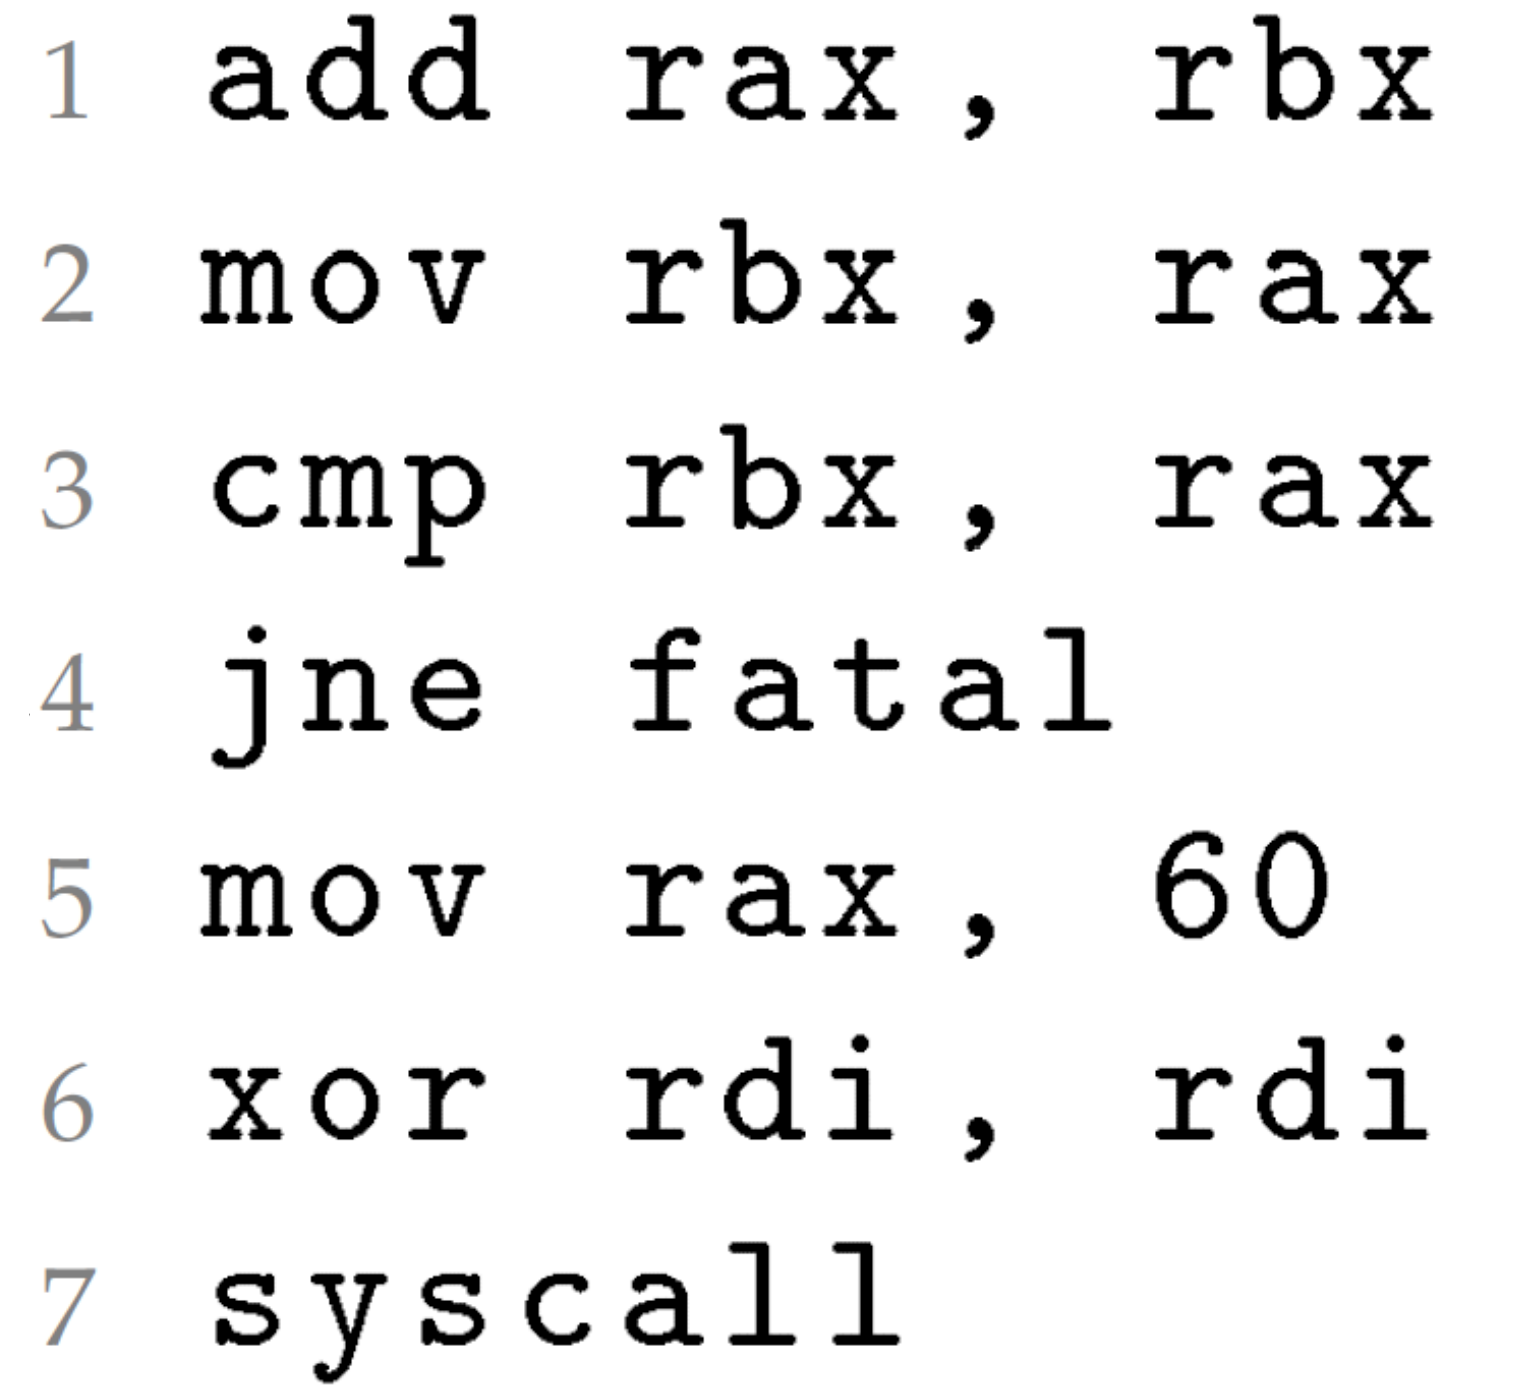
\includegraphics[width=0.4\linewidth]{basic_block}
				\caption{Before Basic Block Creation}
				\label{fig:basicblocks-before}
			\end{subfigure}
			\begin{subfigure}[b]{.5\textwidth}
				\centering
				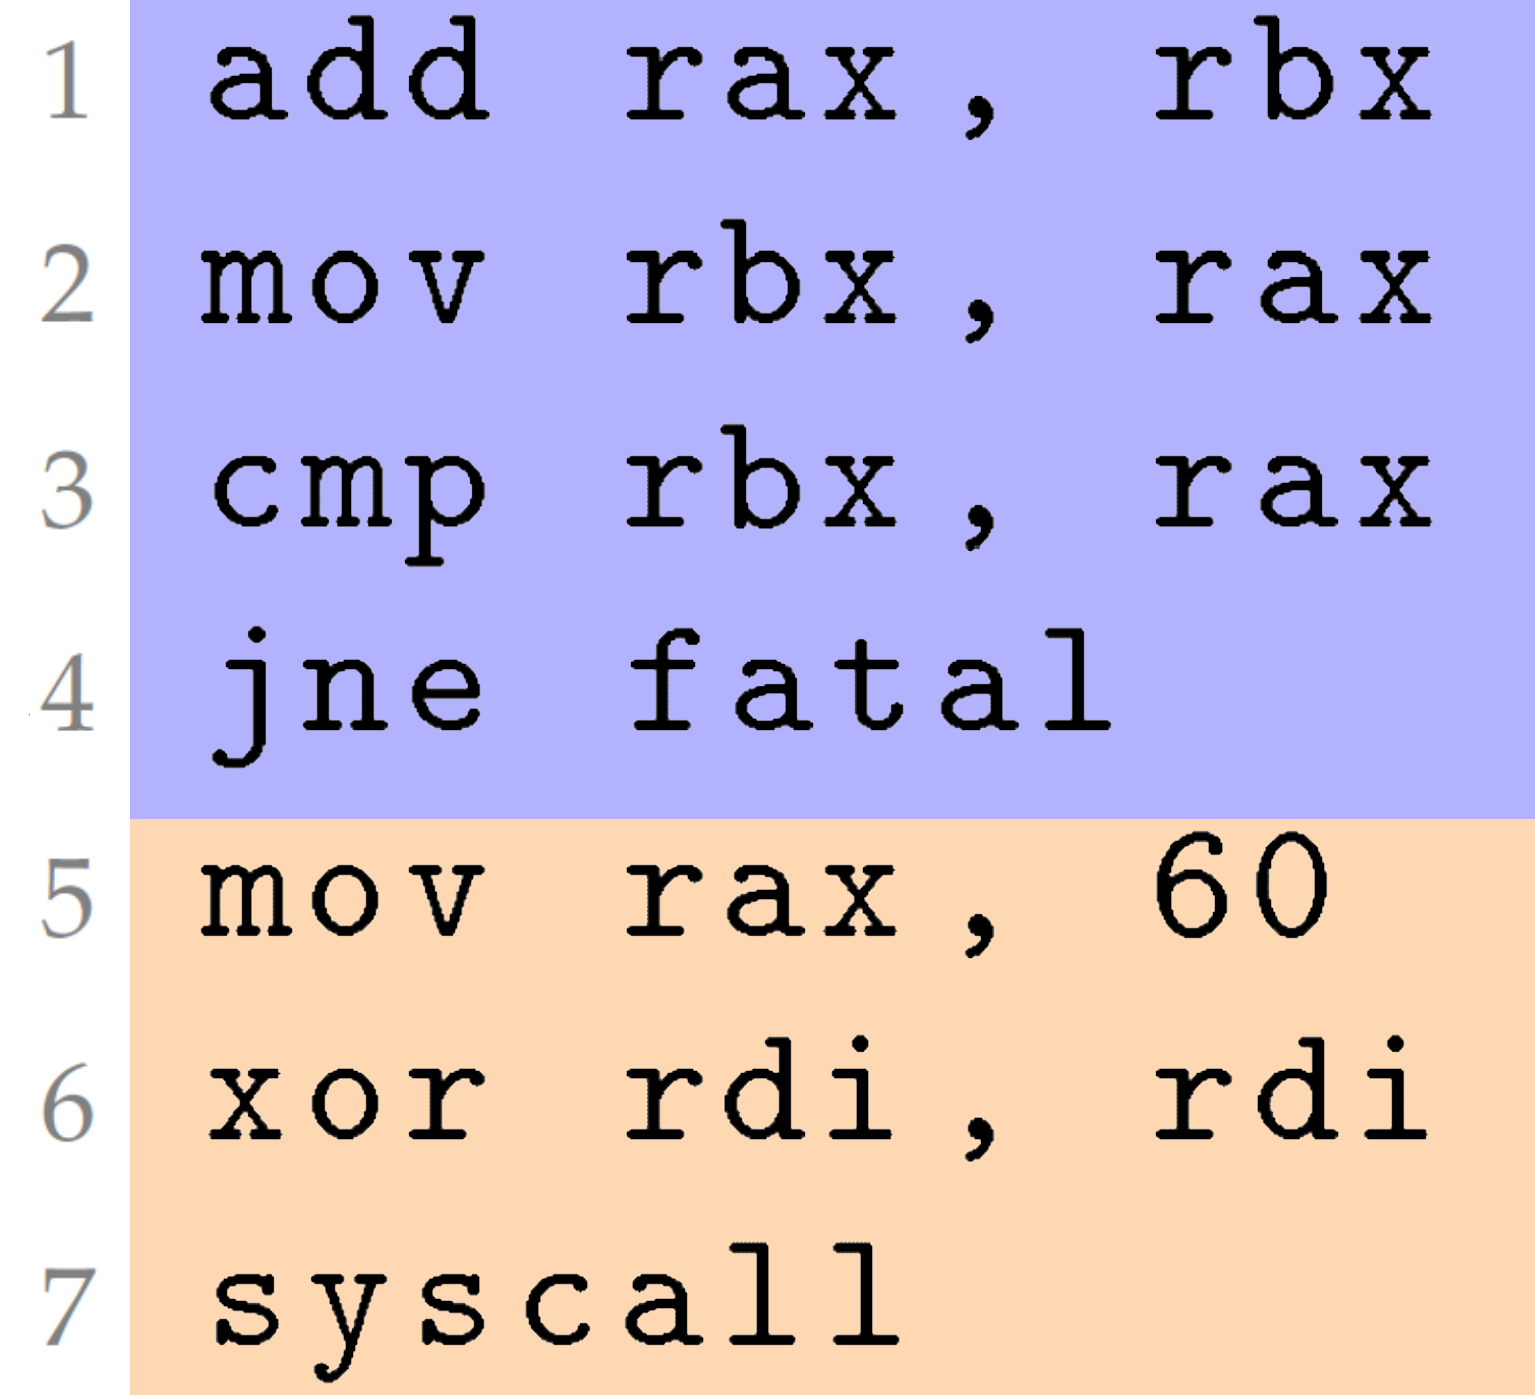
\includegraphics[width=0.4\linewidth]{basic_block_colored}
				\caption{After Basic Block Creation}
				\label{fig:basicblocks-after}
			\end{subfigure}

			\caption[Basic Block Separation]{An example on the scope of basic blocks (in x86-64 assembly).}
			\label{fig:basicblocks}
		\end{figure}

		The final instruction of every basic block can be understood as a link, or a reference to another block (or the end of execution). With this interpretation of links, each executable can be depicted as a set of multiple basic blocks linked with each other. Those links can either be \emph{static}  or \emph{dynamic}. Static links have a constant target, such as a direct jump to an address (e.g. \texttt{jmp label}). Whereas dynamic links have a variable target, for example an indirect jump (e.g. \texttt{jmp rax}).
		
	\subsubsection{Linking Blocks}
	\label{Block Chaining}
		Since the actual target (i.e. the address of the executable RISC-V code) is (initially) unknown, the destination has to be evaluated at runtime by the host. The first time a static link is accessed, the host evaluates the target address once and modifies the link so that it points directly to an instruction in a block. \emph{Block Chaining} describes this concept of permanently connecting two statically linked blocks by evaluating the destination only once at translation time.
	
		Dynamic links on the other hand are always indirect: Since the target depends on an external, unknown value (e.g. a register), the target of the link can only be determined by the host. This means, that the address has to be evaluated every time the link is taken.
		
		Chaining blocks may drastically save time in hot paths since the translator only has to be called once. Additionally, this allows for the execution of multiple basic blocks at once, without further intervention of the host.
		
	\subsubsection{Super Blocks}
	Basic blocks with multiple exit points and as single entry are called \emph{super blocks}. With these, conditional jumps do not necessarily have to end the block, allowing the execution of more code without intervention of the host. If two super blocks reference the same basic block, it may be better to duplicate the generated code instead of adding additional jumps \cite{smith2005virtual}. With duplicated code, both super blocks can be larger and function independently.

\subsection{Code Storage}
\label{code storage}
After a block of code has been translated, it must be decided how long it should be stored. Many programs run sequentially, meaning that except for loops it is rare for already executed parts to be revisited. One option for storing translated code is to implement a so-called code cache. By deleting older sections of translated code on the assumption that they will not be executed again, a DBT can save a lot of memory depending on the size of the guest program.

When storing translated code indefinitely on the other hand, the target of a jump is consistent, as the addresses of instructions are permanent. Since the code translation process itself causes some overhead, a permanent code storage may drastically reduce the number of translations. The reallocation of already translated code has to be handled with special care in this configuration, as all jumps to already translated blocks become invalid.

Another situation the code store must handle is a jump to an arbitrary instruction of a basic block instead of the beginning. This poses no problem if blocks are stored in a way that allows access to the addresses of individual translated instructions\footnote{This is not entirely trivial since a single x86-64 instruction may be translated into multiple RISC-V instructions.}. If, however, this is the first time that the basic block is accessed, it has to be translated first, meaning that the part before the jump target will be left untranslated. If the guest ever tries to access that part, the DBT will have to either re-translate the whole block and store it twice, relocate the already translated part to join it with the new part (and fix any jumps that target that block), or add a jump to the old part at the end of the new one.

\subsection{Execution}
Executing the guest program concurrently with the host is a rather complex process. Since guest and host could interfere with each other, countermeasures have to be taken to separate the two programs. Fully hiding the host from the guest is not feasible since this would cause a lot of performance overhead. The aim is to run the guest and host in parallel without issues during execution. 

	\subsubsection{Context Differentiation}
	\label{context}
		% Different registers
		% Different stacks
		Unlike in emulation where the guest program is always completely encapsulated by the emulator, a program executed by dynamic binary translation takes full control of the CPU. It will not only change values in registers and memory but also expect these changes to persist between jumps. Unless the host architecture has an absolute abundance of registers to the point where the register space can be split between guest and host (and usually it does not), this necessitates the DBT to keep track of the guest state; store it when the guest reaches a dynamic link, and restore it once execution can continue.
		
		Another essential part is the stack. Unlike registers, this resource could be shared between guest and host by letting the guest operate on the lower half of the host's stack, but this would allow the guest to potentially invalidate the host's stack (e.g. cause a stack overflow). For this reason, it is usually a good idea to allocate a separate stack for the guest.
		
		The combination of those two parts, the stack and all registers, make up the \emph{context}. Guest and host each have their own context that has to be kept track of during the execution process.
		
	\subsubsection{Register Mapping}
	\label{register_mapping}
		Since the guest program expects to be able to access any register, the DBT has to map the space of guest registers to the space of host registers and/or emulate them in memory. Fortunately, RISC-V provides more general-purpose registers than x86-64 (ignoring SSE\dots), which allows every x86-64 register to be mapped to a RISC-V register while still leaving some registers unmapped. These unmapped registers are quite important since the translation of complex instructions often requires storing intermediate values. A few registers could even be used to store a pointer to important jump targets, such as the function for context switching.
		
	\subsubsection{Memory Layout}
		% Grundproblem, dass wir zwei verschiedene Speicherebereiche brauchen
		% Mögliche Lösungen: Memory emulieren, oder yolo auf hohe Adresse linken (yolo, weil man Memory-Konflikte mit uns bekommen soll)
		One could create a second process for the guest application, allowing guest and host to exist side by side with two different address spaces. However, this would require not one, but two context switches to transfer control between the guest and the DBT (guest \(\rightarrow\) OS \(\rightarrow\) DBT), which is one of the most expensive operations in dynamic binary translation.
		
		Another approach is to realize that since the guest program is effectively part of the DBT, it can share an address space with it. If the host platform has a larger address space than the guest, one can simply use the addresses not available on the guest platform for the DBT without fear of interference from the guest. If both platforms have the same address space however, memory conflicts could arise.
		
		One method of solving this conundrum is to emulate the guest memory. However, one could run into difficulties if the guest platform has smaller page sizes than the host and (for memory efficiency) multiple guest pages are mapped to the same host page. This becomes problematic if the guest tries to give those pages different memory protection modes. To solve this problem the DBT could decide to be very lenient and give each of the pages the most allowing of the requested protection modes, which can obviously cause problems if the guest is not well behaved. In that case, the only solutions are to either give each page the most restrictive of the requested protection modes, necessitating the DBT to potentially emulate every memory access (slow), or to give each guest page its own host page, which not only requires a lot more memory but also means that the guest's address space is no longer continuous.
		
		A simpler method would be to figure out which part of the address space usually goes unused on the guest platform and map the DBT to those addresses\footnote{If an application relies on this specific address space, it cannot be executed by the DBT without further modification of either the DBT itself or the host application.}. If one was concerned with safety, one could write-protect those pages and start emulating memory if the guest tries to access them.

	\subsubsection{Dynamic Translation}
		% Sprung zu unserem Programm und wieder zurück
		% Context speichern
		% Dispatcher
		In order to allow for the execution of two programs side by side, a mechanism has to be put into place that specifies when and how to switch between them. In a DBT this role is usually taken up by a so-called \emph{dispatcher}.
		
		The basic idea is that if the guest program encounters an operation that interrupts the execution flow, i.e. a link, the guest context will be saved, and the dispatcher is called. The task of the dispatcher is to ensure that execution of the guest can continue. For this purpose, it may just load the address of the requested jump, or it may have to call out to a system call handler or a translator. Once all the necessary steps have been taken, the guest context will be restored, and guest execution may resume.

\subsection{Control Flow}
	Control flow instructions (such as jumps/calls) mark the end of a basic block and may require costly operations like dynamic block linking or flag evaluation.
	
	\subsubsection{Flags}
		\label{approach_flags}
		% nicht wie es bei uns implementiert ist, sondern dass es einen großen Unterschried bei Sprüngen etc gibt.
		% eager (egal bei HW support) / lazy (gut für RISC-V) evaluation Vergleich
		One of the bigger differences between the two architectures of interest to this project is the handling of conditional branching. The way x86-64, along with most other popular architectures \cite{arm, ppc}, implements it is by having a register dedicated to storing information about the result of the last arithmetic operation. RISC-V on the other hand does not store any information about previous (integer) operations, opting to use fused compare-and-branch instructions instead\footnote{RISC-V does have a flags register for floating point operations}.
		
		The obvious solution would be to emulate the x86-64 behavior, meaning that the DBT must manually update a dedicated flags register after every arithmetic operation, so called \enquote{eager} evaluation. Unless there is hardware support, evaluating flags can be quite costly, especially more complex ones like parity. A more efficient albeit less accurate method is to evaluate flags only for the last arithmetic operation(s) before the flags register is read (e.g. before a conditional jump), so called \enquote{lazy} evaluation. Since flags are often set and then immediately discarded, lazy evaluation can save a lot of time while still being transparent to the guest program. The difference between eager and lazy evaluation is illustrated in \autoref{fig:flageval}.
		
		\begin{figure}[htb]
			\centering
			\begin{subfigure}[b]{.5\textwidth}
				\centering
				\begin{lstlisting}[frame=none,xleftmargin=2.7cm]
add rax, rbx
update flags
add rax, rcx
update flags
add rax, rdx
update flags
jcc label
				\end{lstlisting}
				\caption{Eager Flag Evaluation}
				\label{fig:flageval-eager}
			\end{subfigure}%
			\begin{subfigure}[b]{.5\textwidth}
				\centering
				\begin{lstlisting}[frame=none,xleftmargin=2.7cm]
add rax, rbx
add rax, rcx
add rax, rdx
update flags
jcc label
				\end{lstlisting}
				\caption{Lazy Flag Evaluation}
				\label{fig:flageval-lazy}
			\end{subfigure}
			\caption{Comparison of eager and lazy flag evaluation.}
			\label{fig:flageval}
		\end{figure}

	\subsubsection{Jump}
	\label{translating conditional jumps}
	% Flag support wird da benötigt
	% Adresse dynamisch berechnen bei Sprung zu Register -> Sprung zu Programm (z.B.:)
	Since branching instructions could target not yet translated sections of code, they cannot be translated directly but instead a jump to the dispatcher will be generated. Once there, the dispatcher can examine the target and request translation of it if necessary. If the jump is static, the dispatcher may then replace the call to itself with a jump to the (critically) unchanging actual target (see \autoref{fig:jumptranslation}). This context switch can be eliminated by implementing block chaining (see \ref{Block Chaining}). However, if the jump is dynamic, the dispatcher will have to be called every time to ensure the target is translated and executable.
	
	Note that since the following block could depend on flags set in the current block, all flags have to be updated (even for unconditional jumps). The translation unit can use a look-ahead that recursively analysis following blocks to eliminate many of those unnecessary flag updates. This look-ahead is especially useful with x86-64, as most flags are discarded.
	
	\begin{figure}[htb]
	\centering
	\begin{subfigure}[b]{0.33\textwidth}
		\centering
		\begin{lstlisting}[frame=none,xleftmargin=1.3cm]
jmp label
		\end{lstlisting}
		\caption{x86 Input Code}
		\label{fig:jumptranslation-x86in}
	\end{subfigure}%
	\begin{subfigure}[b]{.33\textwidth}
		\centering
		\begin{lstlisting}[frame=none,xleftmargin=1.1cm]
nop
jalr 0, s11, 0
		\end{lstlisting}
		\caption{Initial Translation}
		\label{fig:jumptranslation-beforedispatcher}
	\end{subfigure}
	\begin{subfigure}[b]{.33\textwidth}
		\centering
		\begin{lstlisting}[frame=none,xleftmargin=0.7cm]
addi t0, zero, label
jalr 0, t0, 0	
		\end{lstlisting}
		\caption{Final Translation Result}
		\label{fig:jumptranslation-afterdispatcher}
	\end{subfigure}
	\caption{Process of translating a static jump (\texttt{s11} stores a pointer to the dispatcher).}
	\label{fig:jumptranslation}
\end{figure}
	
	\subsubsection{Call and Return}
		The x86-64 \texttt{call} instruction pushes the return address (the address of the instruction following the call) onto the stack and then jumps to the address specified in the \texttt{call}. The \texttt{ret} instruction pops the return address from the stack and jumps to it. The naive approach to translating these is by translating the \texttt{call} as a push of the return address and a jump to the specified address. A \texttt{ret} would pop the return address and look for the RISC-V code in the code store or translate it, if it's not cached. However, the lookup in the code store is costly and would have to be performed for each execution of \texttt{ret}. Fortunately, there are ways to resolve this issue. 
		
		One of them is to alter the behavior of the \texttt{call} such that it translates the basic block starting from the return address and pushes the address of the generated RISC-V code. \texttt{ret} could then just pop that address and jump to it directly. This approach is fine for most C programs, because they neither read nor modify the return address, but results in undefined behavior if the program relies on such techniques. It also requires storing the translated code indefinitely.
		
		A second option would be to implement a return stack similar to what many modern processors use for branch prediction \cite{arm-technical-reference-manual}. The return stack holds information that is used by \texttt{ret} in two ways:
		\begin{enumerate}
			\item Check if the return address has been altered. In this case \texttt{ret} has to find the code that corresponds to the new return address dynamically.
			\item Find the RISC-V code of the original, unmodified return address efficiently.
		\end{enumerate}
		This information is provided by \texttt{call}, which does not only push the return address onto the guest stack but also additional information onto the return stack.
		
	\subsubsection{System Calls}
	\label{approach_syscalls}
		% Exit Syscall "problematisch"
		% nicht reines durchgeben
		% Indizes der Syscalls verändern sich
		% Syscall könnten theoretisch unseren Heap zerstören (bei z.B. remapping, brk)
		Communicating with the operating system/kernel is an essential operation, but the interface greatly differs between architectures. While a special \emph{syscall} instruction may be a constant, the system call index, the expected arguments or even the existence of such a system call is far from invariant. For example, the \texttt{open} system call (index 2), which is supported in x86-64, has been replaced by \texttt{openat} (index 56) in RISC-V; numbering also differs.
	
		Additionally, some system calls could have highly destructive effects on the DBT, for example \texttt{exit}, which would not allow the DBT to clean up after itself, or \texttt{brk}, which could destroy the DBT's memory. As such, the DBT needs to intercept any system calls and emulate them appropriately, effectively acting as the operating system as far as the guest is concerned.
	
\subsection{ELF}
	The Executable and Linkable Format (ELF) is a file format used by Linux and Unix like systems to distribute binaries and dynamically linked libraries. Even though the ELF format is not originally from Linux, most binaries nowadays produced on modern Linux systems will come in the form of an ELF file. An ELF file contains everything required to run the included binary. This includes various information about the required environment (e.g. architecture, stack size) as well as the binary itself and data required by the binary. To execute an ELF binary, the file only needs to be loaded partially into memory. 
	
	\subsubsection{Sections} 
	The core principle of the ELF format is the concept of sections. Sections are primarily used in the linking process to link multiple ELF files together. A single ELF file can contain many sections. A section consists of a name, a virtual address and size, which describe where the section should reside in memory once the ELF file is loaded. It also contains a file offset and file size which describe where the data reside within the file. Additionally, it contains attributes which describe whether the contents should be flagged as readable, writable, and/or executable or whether the section contains any information in the file, and if it should be loaded into memory in the first place.
	
	There are some default names (e.g. \texttt{.text}, \texttt{.bss}, \texttt{.symtab}) of which the sections are expected to hold the information described by their name. By default, the text section contains the executable code and the bss section should contain uninitialized data (it is flagged as containing no data in the file, and only in memory). The symtab section contains a list of symbols defined by the binary. A symbol is a pair of a name (e.g. function name or variable name) and an address, which describes where to find it. But every compiler can add as many sections as required.
	
	\subsubsection{Program Headers}
	The ELF format also describes the program header: every ELF file contains a list of program headers. They simplify the work of loading the binary into memory when trying to execute it. Every program header contains virtual address and size information, as well as file offset information. The program headers are used for executing a binary: when the program headers have been loaded into memory it is ensured that all necessary data required to run the binary are in the memory. The program header also contains necessary information required to potentially load shared libraries and to dynamically link the binary to these. 
	
	\subsubsection{Shared Libraries}
	Most ELF files do not contain all the code required to run the binary or all the data required. This is because code and data might be shared between multiple binaries. Thus, they have to be dynamically linked for the initial binary to work properly. The program header list in the ELF file contains entries, which hold the name of required ELF file(s) as well as the name of the interpreter required. The interpreter processes the information about the dynamic linking and handles the entire linking process. Those required binaries might also depend on (possible multiple) other ELF files. For the program to be executed properly, all these requirements have to be satisfied. In order to link those ELF files, the program headers are required, as they contain special entries. These entries tell the interpreter, where the addresses of other ELF files and some of their symbols have to be written to.

\section{Documentation of the Implementation} % 12 Seiten
Our goal in navigating the space of possible designs was first and foremost to ensure that the product would be highly performant. To achieve this, we chose to store translated code indefinitely, which allowed us to make certain optimizations when translating jumps and simplified the design overall. Flags are evaluated lazily over the scope of multiple blocks. We do not emulate memory for the guest and link oxtra itself to a high, usually unused address instead. Blocks similar to super blocks but with multiple entry points are used as base unit of translation to reduce the number of links to other blocks.

To ensure we met the time constraints and for our programming pleasure we chose an object-oriented approach in C++, allowing us to divide our source code into classes for ease of navigation and to work concurrently on the project without fear of intersection.

To decode x86-64 instructions, we have decided to use fadec\footnote{\url{https://github.com/aengelke/fadec} (visited on 12/10/2019)}, a 32 and 64 bit compatible decoder, written in C and adapted by us to be object oriented for easy use in oxtra. For logging, we use a small wrapper for fmt\footnote{\url{https://fmt.dev/latest/index.html} (visited on 12/10/2019)}.

\subsection{Architecture Overview}
	The implementation of the translation process is abstracted by the dispatcher. To start the translation of a binary only a \texttt{Dispatcher} object has to be created, which internally manages all the other components of the architecture. To initiate the execution, \texttt{run} is called on the dispatcher object. \texttt{run} returns the return value of the translated program, once the execution is finished.

	\subsubsection{Internal Block Structure}
	To translate code sections, oxtra splits instructions into chunks which are advanced deviations from super blocks. Those \emph{blocks} are defined as a list of consecutive operations up to the next block ending instructions. Block ending instructions are: \texttt{jmp}, \texttt{call}, \texttt{ret} and \texttt{syscall}. This structure similar to super blocks means, that a block may contain multiple exit points (e.g. conditional jumps). Due to the internal structure and capabilities of the implementation, a block can also have multiple entry points upon creation. This renders these blocks incapable of being called basic blocks or super blocks, as they have a single point of entry per construction.

	\subsubsection{Environment Initialization}
		% in english, long dashses do not have a space
		The initialization process of oxtra is rather straightforward and is illustrated in \autoref{fig:lifecycle-initialization}. Initially, the arguments are parsed and processed with the use of \emph{argp}---not only the arguments that control oxtra itself but also those that will be passed to the guest application.
		
		Afterwards, the ELF file itself will be processed---thoroughly explained in \ref{documentation_elf}---which breaks down into three major steps: opening the elf file, ensuring correctness of essential values, and unpacking the elf file into memory for easy processing.
		
		In the next step, the guest is initialized by setting the context (see \ref{context}) according to the x86-64 System V ABI\footnote{The Application Binary Interface defines low level requirements and behavior specific to a kernel and an architecture.}, mainly allocating a stack for the guest and pushing key values (e.g. argument count, arguments, environment variables \dots) onto it \cite{systemv}. With the guest prepared, oxtra can switch to the new context and start translating the initial code block.
		
		\begin{figure}[htb]
			\centering
			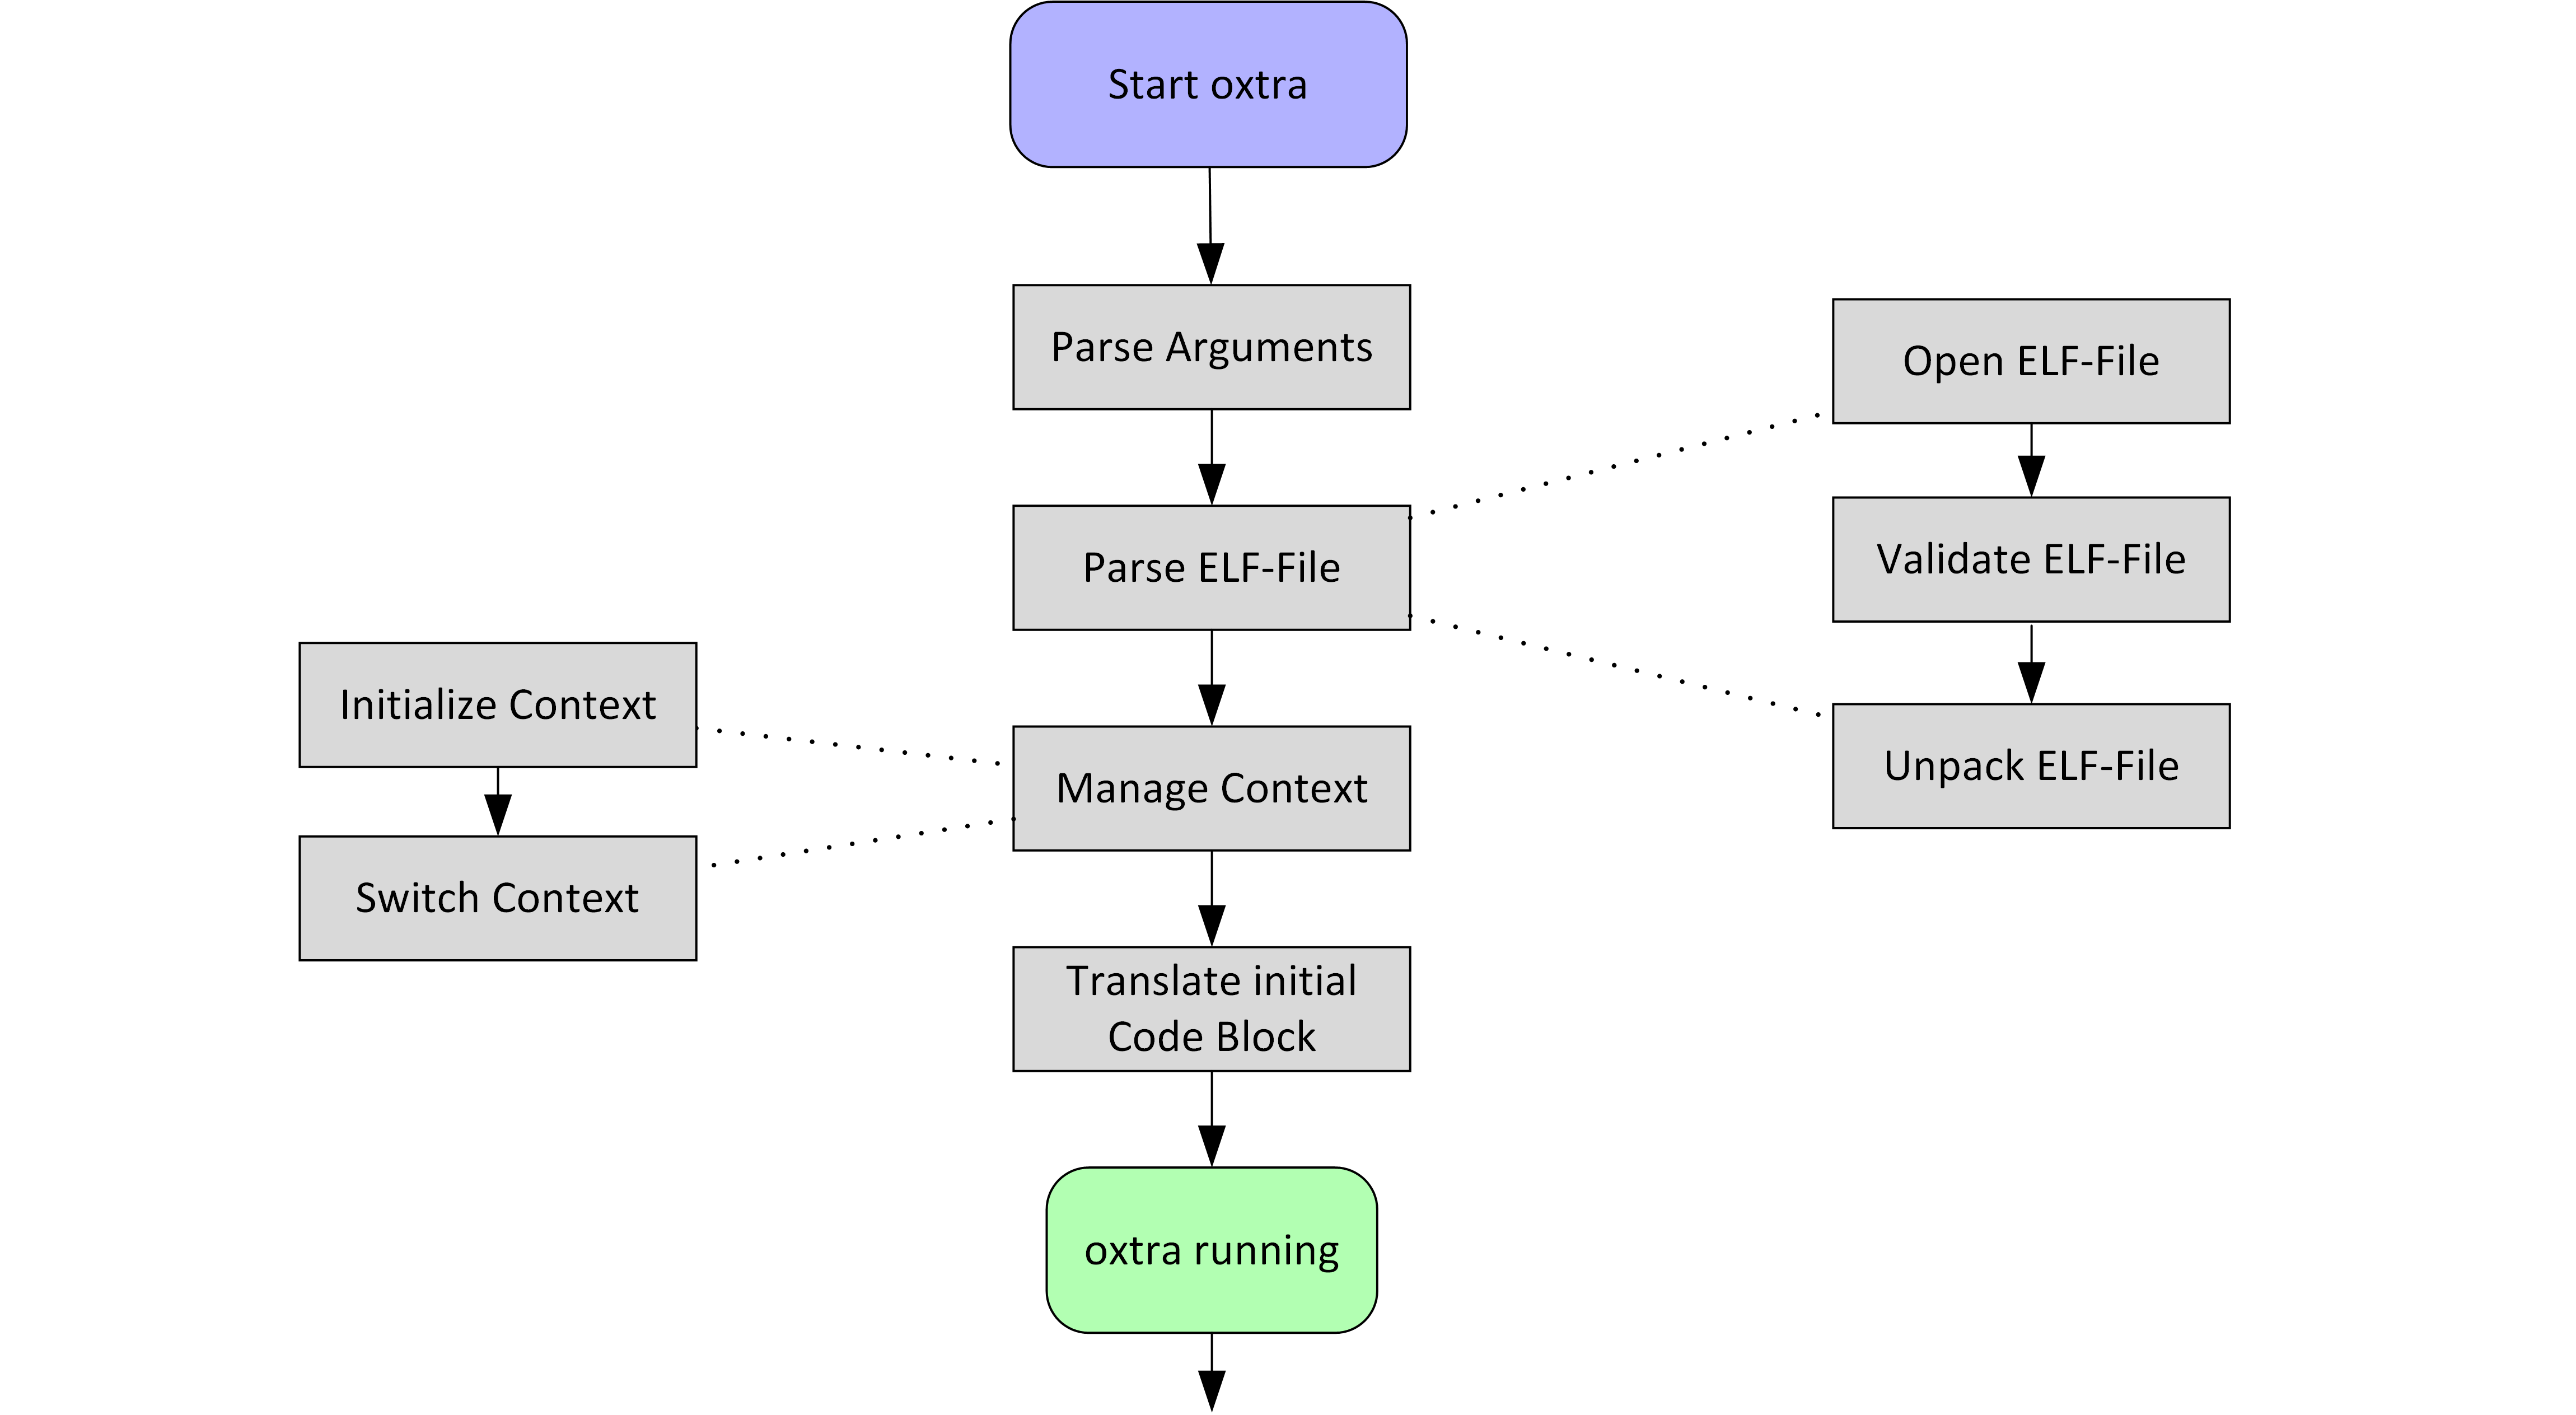
\includegraphics[width=1.0\linewidth]{architecture/lifecycle-initialization}
			\caption[Runtime Initialization]{Initialization of the runtime environment and preparing oxtra for execution.}
			\label{fig:lifecycle-initialization}
		\end{figure}
	
	\subsubsection{Core Processing Cycle}
		After oxtra has been successfully initialized and the first block translated, the translation loop has started. This life cycle, illustrated in \autoref{fig:lifecycle-processing}, begins by executing an initial block, possibly followed by multiple statically linked blocks (see \ref{Block Chaining}).
		
		Eventually, a target of a block cannot be statically evaluated (e.g. an untranslated block or the target is stored in a register), forcing the guest to give control back to the host. After the context of the guest has been stored, the host can fully take over (marked by the dash-dotted rectangle).
		
		The Code Manager ensures that the target address has already been translated. If this is not the case, the block beginning with this address will be translated and stored. After this procedure, the address of the actual RISC-V instruction can be passed to the guest and used as the starting point for further execution. In our implementation, any arbitrary instruction in an already translated block can be referenced and used as a starting point, without the need to duplicate code. 
		
		If the final link in a chain of blocks is a static link, the last block and the new block will be chained \emph{statically} by replacing the switch to the host with a jump directly to the next block (see \ref{Block Chaining}). If it is a dynamic link, the address has to be reevaluated every time the link is taken (see \ref{translating conditional jumps}).
		
		Eventually, an exit system call (or an error) is encountered, marking the end of the execution process and causing the guest to stop. If the error was detected (not all segmentation faults are detected), the context of the host will be fully restored. Finally, the exit code of the guest is returned by the host itself causing the guest and the host to be stopped. 
		
		\begin{figure}[htb]
			\centering
			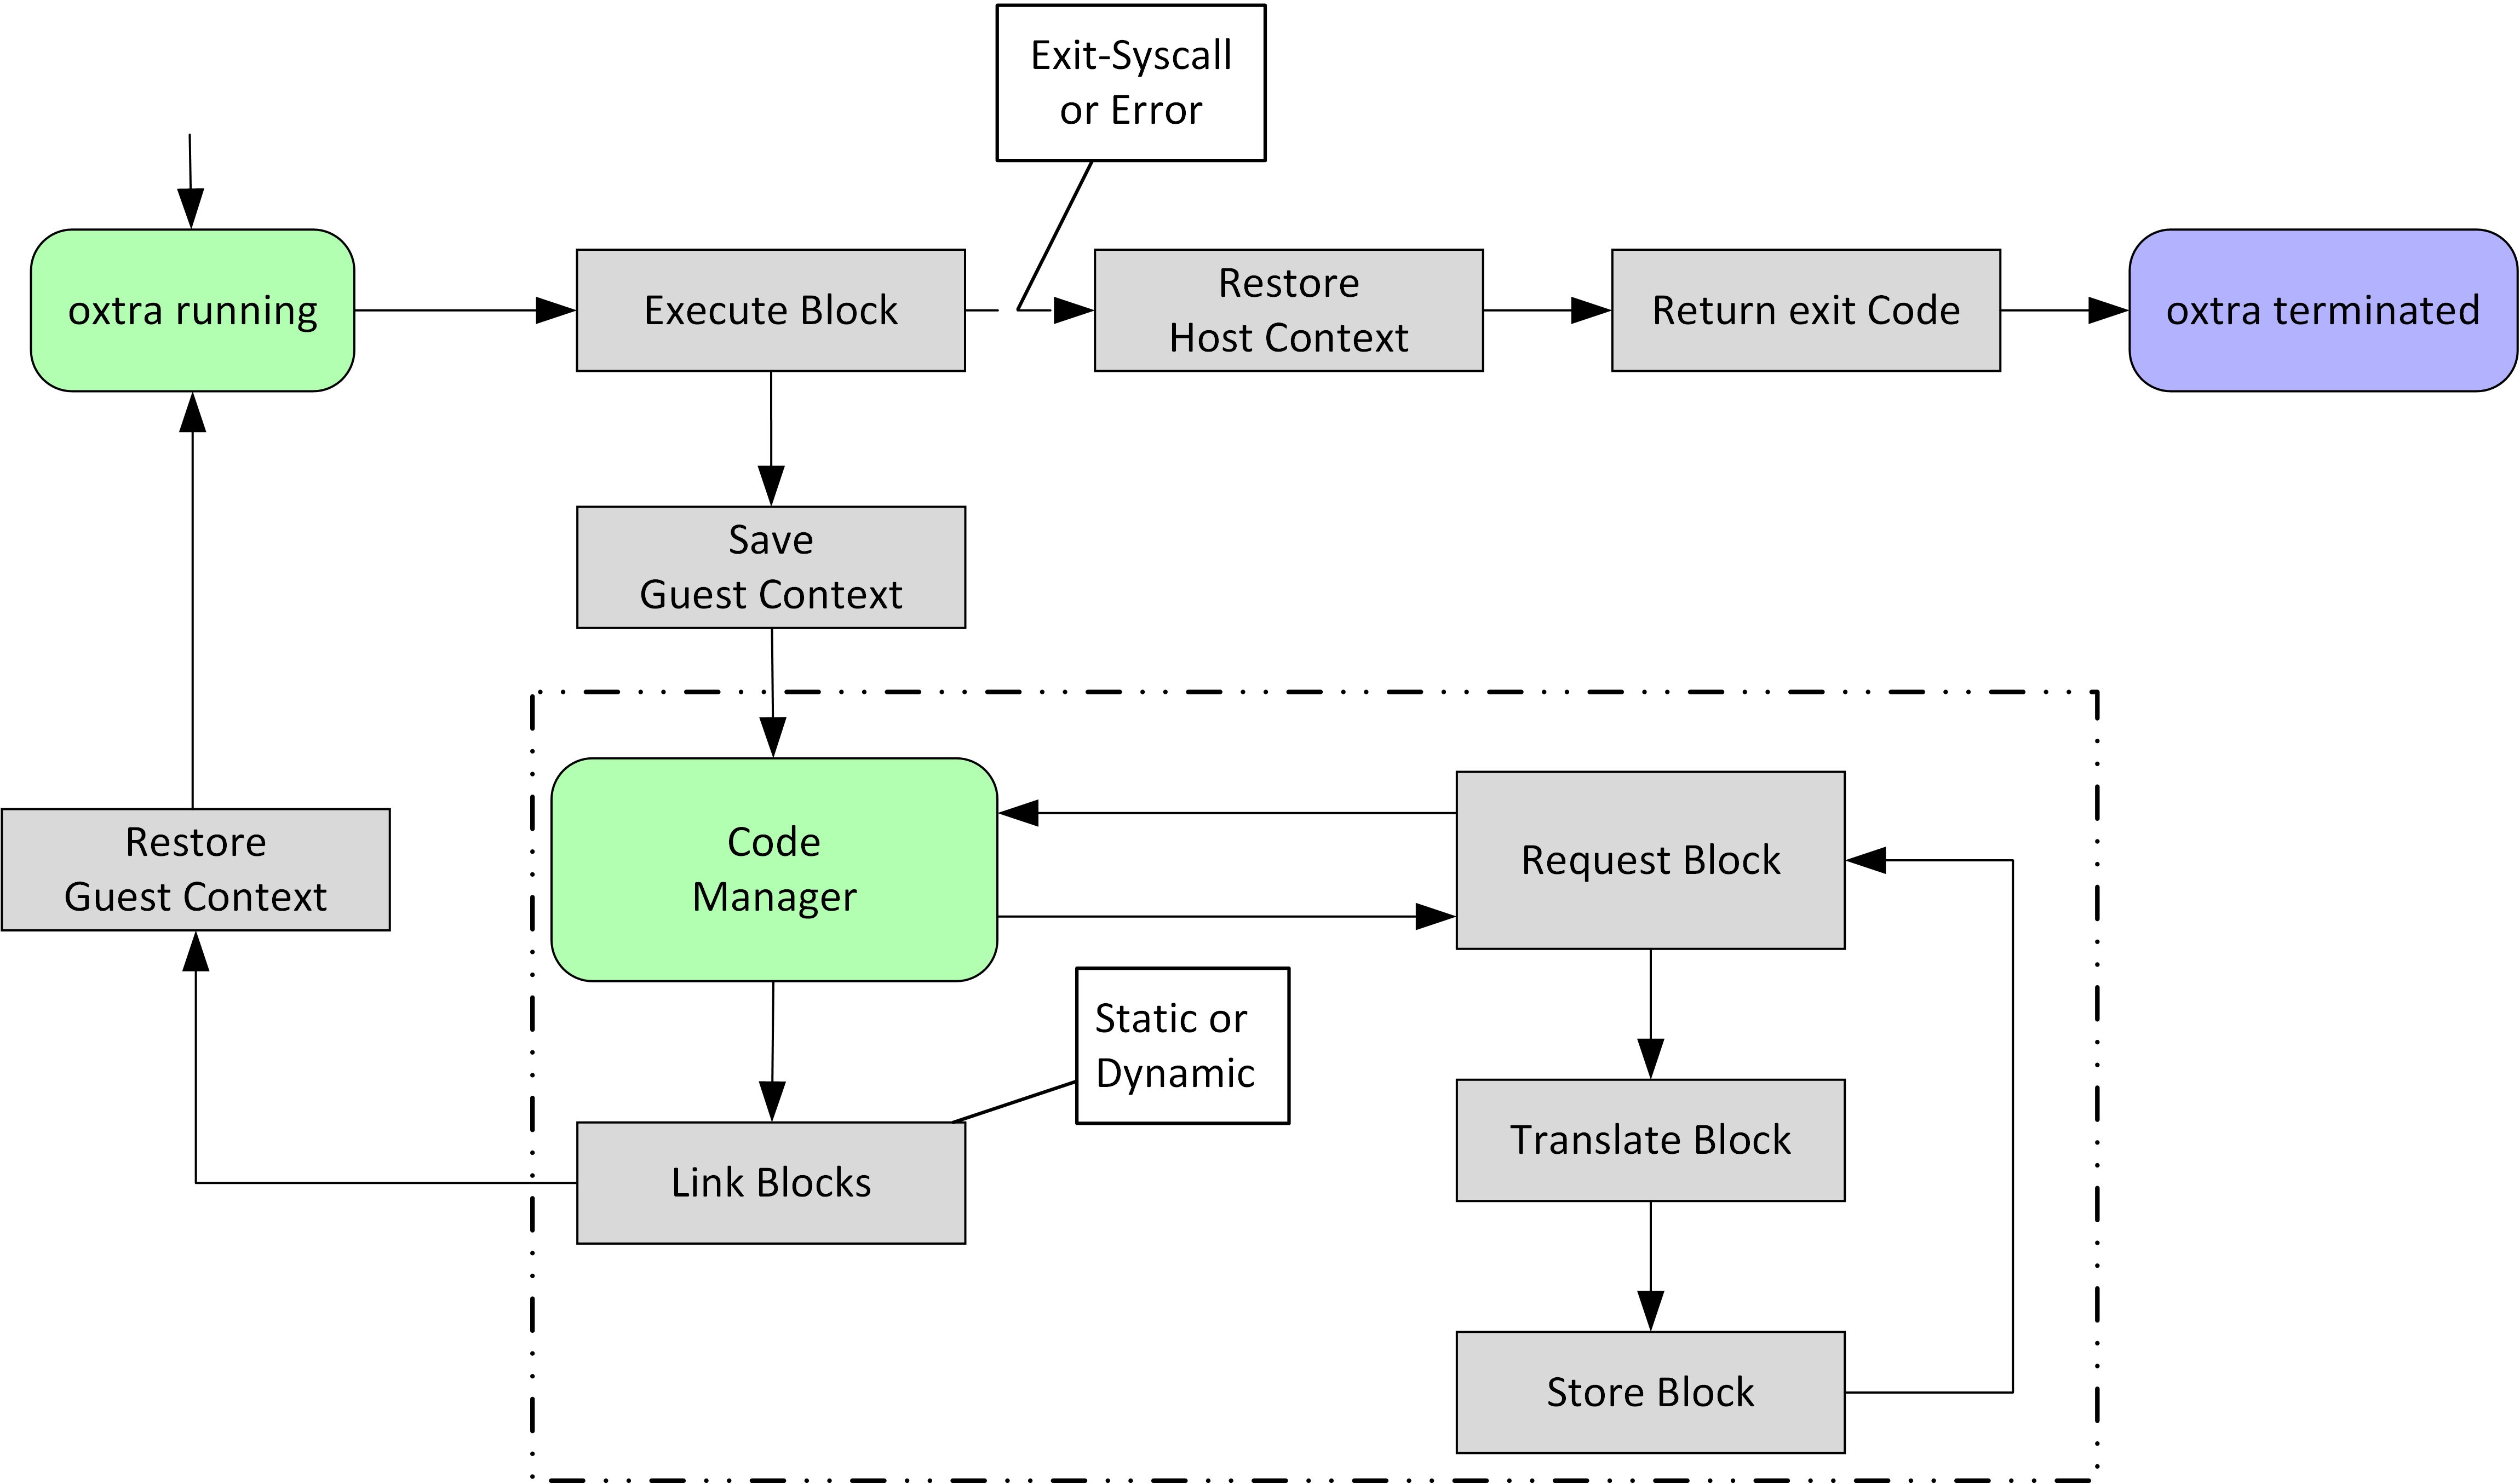
\includegraphics[width=1.0\linewidth]{architecture/lifecycle-run}
			\caption[Instruction Processing]{Processing cycle responsible for translating, executing, and storing instructions.}
			\label{fig:lifecycle-processing}
		\end{figure}
	
	\subsubsection{Component Overview}
		For translating and executing blocks, oxtra requires three core components that have been illustrated in \autoref{fig:component-overview}.
		
		\paragraph{The Dispatcher} implements the interface between the guest and host. Whenever the guest gives control back to the host, a method of the dispatcher is being called. Those methods control the main execution flow like the translation of blocks or the mapping and emulation of system calls. This means that the Dispatcher essentially controls the host.
		
		\paragraph{The Code Generator} translates blocks and generates RISC-V instructions accordingly. Additionally, it controls the flag evaluation process, mainly consisting of selecting instructions that should set flags (lazy evaluation) and ensuring that flags are consistent over multiple blocks.
		
		\paragraph{The Code Store} saves and manages previously translated blocks with a simple paging mechanism. Before generating a block, the Code Generator queries the Code Store whether this block has already been translated. With the current implementation, this caching mechanism does not allow reallocation or deletion of blocks (see \ref{code storage}).
		 
		\begin{figure}[htb]
			\centering
			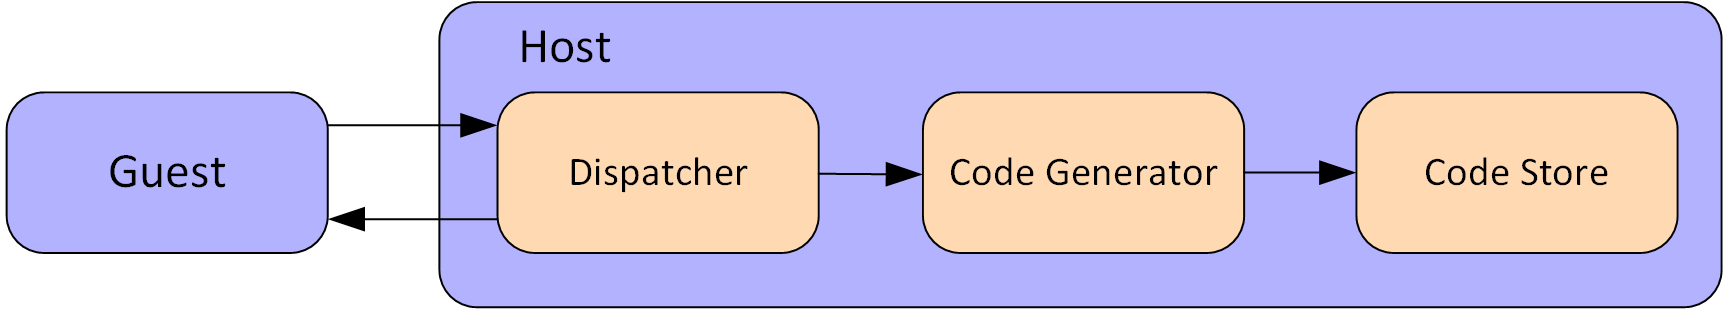
\includegraphics[width=0.75\linewidth]{architecture/component-overview}
			\caption[Component Overview]{Core components participating in the translation and execution process.}
			\label{fig:component-overview}
		\end{figure}

\subsection{In-Depth Architecture}
	The architecture described in the previous sections simplifies many aspects and is meant to be a starting point. It either ignores the underlying system that composes a higher-level component or leaves out some (rather) important parts. The UML class diagram illustrated in \autoref{fig:uml-architecture} fills this gap and shows the actual dependencies and associations between the components/systems, while only leaving out smaller details.
	
	\subsubsection{Dispatcher}
		The two purposes of the main method are to create the dispatcher with all required references (namely elf and arguments) and invoke the translation and execution process by calling \texttt{run}. Once this procedure has been initiated, the dispatcher prepares the \texttt{ExecutionContext} which stores important values for the host/guest (e.g. the contexts), and the execution process (e.g. flag information). Afterwards the first block can be translated, the context switched, and the execution process started.
		
		The dispatcher is not only responsible for setting up the guest, but also functions as the central access point for the guest: whenever supervision by the host is required, a specific method of the dispatcher will be called that decides the further flow of execution. This means that the dispatcher has special entry points for handling system calls and linking blocks that will be called from the generated RISC-V assembly. 
	
	\subsubsection{Code Generator}
		The code generation system (\texttt{CodeGenerator} and its dependencies) provides two main interfaces: translating a given guest address until the end of a block is encountered and chaining previously translated blocks. In theory, this code translation process seems quite straightforward, but many functioning parts are required for the process to work properly.
		
		One essential part is the \texttt{CodeBatch}, which provides a unified way for the instruction classes to store generated instructions. It also allows adding placeholders (e.g. \texttt{nop}s), that are replaced later (e.g. for conditional jumps). Further, the usage of \texttt{CodeBatch} as a generic construct allows us to exchange it with a \texttt{DebuggerBatch} that adds additional instructions and notifies the Debugger of new operations. 

		To translate x86-64 to RISC-V, every x86-64 instruction is implemented in its own class that inherits from \texttt{Instruction}, or, should it make implementation easier, from \texttt{UnaryOperation} or \texttt{BinaryOperation}\footnote{Some similar instructions share a common class (e.g. mul, and imul).}.
		
		In the core translation cycle, the \texttt{decode\_instruction} method of the \texttt{CodeGenerator} is repeatedly called. To decide which x86-64 fadec instruction corresponds to which actual implementation, the \texttt{InstructionTransform} is used. This class provides a mapping method that transforms x86-64 instruction into our implementation. The specific instance then adds RISC-V instructions to the \texttt{CodeBatch}, which are then stored in the \texttt{CodeStore} by the \texttt{CodeGenerator}.

	\subsubsection{Code Store}
		Three essential pieces of information need to be stored for the \texttt{CodeStore} to manage the executable code properly: the actual RISC-V code that can be executed, the address of the x86-64 instructions, and the number of RISC-V instructions per x86-64 operation. With this information, the code can not only be stored but also searched for with \texttt{find(addr)}. By storing the length of every x86-64 instruction, this interface also allows for finding addresses \emph{in} already translated blocks (instead of only finding the address of the start of a block).
		
		It is worth noting that for a block to be executed linearly and as a whole, the code has to be stored \emph{sequentially}. For this we implemented \texttt{StaticList} that can guarantee sequential storage for a given set of data. Additionally, this list also ensures that already translated addresses are not reallocated, preventing blocks from becoming invalid over time.

	\begin{figure}
		\centering
		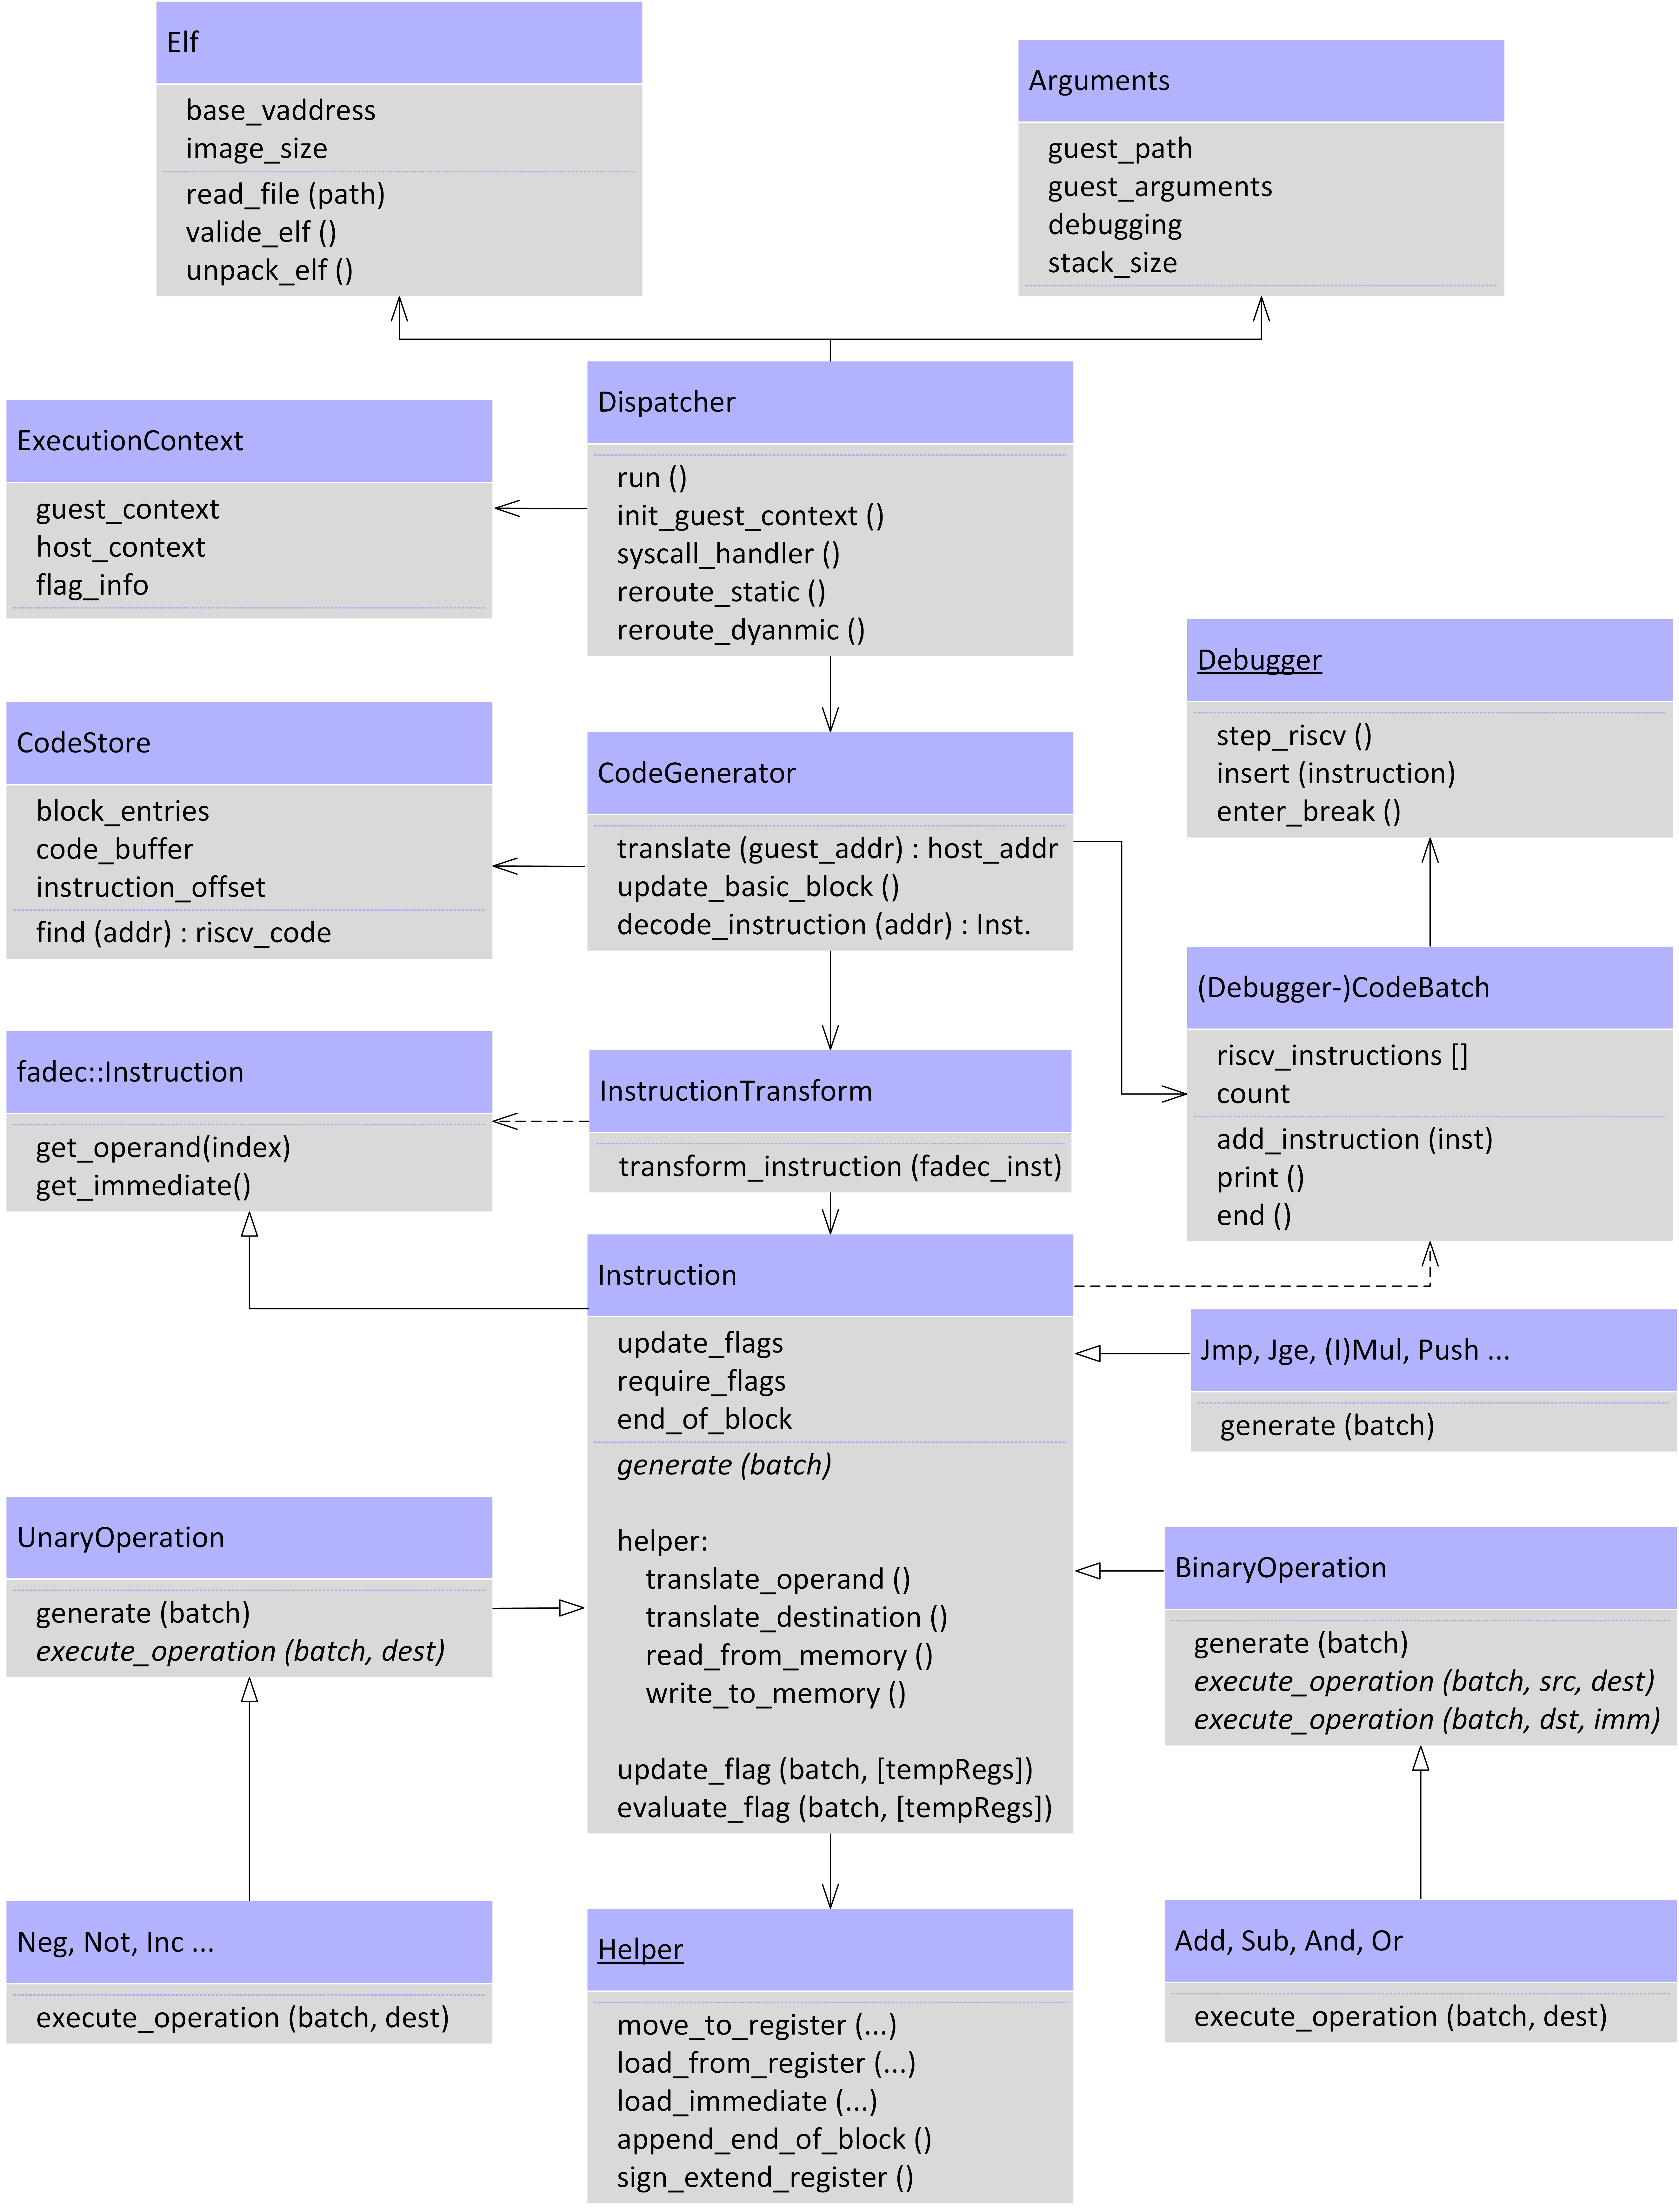
\includegraphics[width=1.04\linewidth]{architecture/uml-architecture}
		\caption[In-Depth UML Architecture]{Architecture of oxtra represented as an UML class diagram.}
		\label{fig:uml-architecture}
	\end{figure}

\subsection{Register Mapping}
As previously mentioned, oxtra maps every x86 register to a RISC-V register. The mapping used in oxtra is illustrated in \autoref{fig:register-mapping}. This mapping has not been chosen arbitrarily, but ensures that the registers for system calls do not have to be moved or altered. The registers \texttt{s1}, \texttt{s8}, \texttt{s9}, \texttt{s10}, and \texttt{s11} store addresses required for execution and will be explained in the following sections. 
\begin{figure}[H]
	\centering
	\begin{subfigure}[b]{.5\textwidth}
		\centering
		\begin{tabular}{|c|c|} 
			\hline
			\textbf{RISC-V Register} & \textbf{Purpose}\\
			\hline
			a7 & rax \\
			a6 & rcx\\
			a2 & rdx \\
			s2 & rbx \\
			sp & rsp \\
			s0/fp & rbp \\
			a1 & rsi \\
			a0 & rdi \\
			a4 & r8 \\
			\hline
		\end{tabular}
	\end{subfigure}%
	\begin{subfigure}[b]{.5\textwidth}
		\centering
		\begin{tabular}{|c|c|} 
			\hline
			\textbf{RISC-V Register} & \textbf{Purpose}\\
			\hline
			a5 & r9 \\
			a3 & r10 \\
			s3-s7 & r11-r15 \\
			s1 & Return Stack \\
			s8 & Call Table \\
			s9 & TLB \\
			s10 & Jump Table \\
			s11 & Context \\
			t0-t6 & Temporary \\
			\hline
		\end{tabular}
	\end{subfigure}
	\caption[Register Mapping]{Specification on the usage of the 31 available registers in RISC-V.}
	\label{fig:register-mapping}
\end{figure}

\subsection{Translating Instructions}
	The primary translation routine consists of four steps: Initial validation, instruction mapping, flag prediction, and code generation.
	
	\paragraph{Initial Validation} ensures that the upcoming address is valid and has not been translated yet. First, the upcoming address is validated against the ELF file to ensure that the new target address is valid and inside the text section. If the address is valid and has not been translated before, oxtra will extract the address of the next upcoming block, which has already been translated, from the \texttt{CodeStore}. Using this upcoming address, the main three processing components are executed.
	
	\paragraph{Instruction Mapping} is the process of decoding the instructions and mapping them to actual instruction classes capable of generating RISC-V code. This process is repeated for every instruction until either a block ending instruction (e.g. \texttt{ret}, \texttt{call} \dots) is found, or an already translated block is encountered. Stopping at a previously translated block ensures that every instruction is translated only once (see \ref{code storage}). 
	
	\paragraph{Flag Prediction} determines which flags each instruction must update. In order to achieve this, two additional pieces of information are stored for each instruction: the flags that the instruction requires for execution (e.g. \texttt{adc} needs the carry flag) and the flags that the instruction alters (e.g. \texttt{inc} updates all flags except the carry flag). To predict which instruction must update a certain flag, the instructions are iterated in reverse order. By iterating in reverse, the instructions which read the flags are encountered before the instruction which would have to update the flag. These are then marked as having to update the given flag. Thus, only the necessary instructions will update any given flag. Additionally, to ensure that flags are consistent over blocks, the instruction that ends the block determines which flags are further required. If the target block is statically linked, the flags will be analyzed recursively (up to a maximum depth) with the next block, reducing the number of evaluated flags. With dynamic links, all flags have to be updated as the next block and it's required flags cannot be predicted.
	
	\paragraph{Code Generation} produces the executable RISC-V code and can be started once the required flags for every instruction are known. Oxtra then begins to translate all instructions inside the current block by calling the \texttt{generate} function of each \texttt{Instruction}. In conjunction with the code store, these translated instructions are written sequentially into memory. \\
	
	\noindent Once all instructions have been translated and stored permanently, the starting address of the newly translated block is returned, and execution can continue.

\subsection{Jump Table}
	\label{Jump Table}
	Jumping to an arbitrary address on RISC-V involves loading the address into a register and then jumping to that address with \texttt{jalr} (possibly up to eight instructions). There are a few addresses that are constantly jumped to during translation and execution such as the methods for statically or dynamically linking blocks, the system call handler or carry and overflow evaluation functions (see \ref{documentation_flags}). These are stored in the jump table.

	The jump table consists of \texttt{jal} instructions which add a signed 20 bit offset to the address of the next instruction and then jump to it, effectively allowing for jumps into a 1 MiB large region around the program counter. The address of the jump table is stored in a register (see \ref{register_mapping}) and jumped to with just one \texttt{jalr} instruction, which encodes a signed 12 bit offset. This jumps to an entry in the jump table which in turn jumps to the corresponding function. The return address points to the instruction after the \texttt{jalr}.

\subsection{Evaluating Flags}
	\label{documentation_flags}
	Oxtra implements lazy flag evaluation, which means that flags are not calculated for every instruction but rather only when they are needed (e.g. in conditional jumps) (see \ref{approach_flags}). This mechanism is implemented by the \texttt{Instruction::update\_flag} and \texttt{Instruction::evaluate\_flag} methods. Oxtra only supports the \texttt{carry}, \texttt{overflow}, \texttt{sign}, \texttt{parity}, and \texttt{zero flag}. The other flags are ignored, as they are either meant for system programming or practically deprecated. The only other flag, which might be interesting is the \texttt{direction flag}. By not implementing the two instructions that can update the \texttt{direction flag} (\texttt{std}, \texttt{popf}), it is ensured that the flag cannot be set, which would lead to undefined behavior.
	An instruction that modifies a flag calls the \texttt{update} method and an instruction that reads a flag calls the \texttt{evaluate} method for that flag. The \texttt{update} methods store values in the \texttt{ExecutionContext} and the \texttt{evaluate} methods read the values from there and calculate the state of the flag. For the zero, sign, and parity flag the \texttt{update} methods store the result of the operation that updated the flag (e.g. the x86-64 \texttt{add} instruction stores the sum of the two input values). The carry and overflow flag calculation depends on the type of operation that updated the flag, so the \texttt{update} methods store an offset into the jump table where the corresponding evaluation function is located, in addition to two input values. The carry and overflow \texttt{evaluate} functions now load this offset and jump into the jump table to the concrete evaluation function.

\subsection{Intermediate Representation}
	Oxtra has been designed in a way that allows fast and easy implementation of new instructions. Because x86-64 has hundreds of instructions, oxtra is not nearly capable of translating all of them. Most of the core instructions of x86-64, (i.e. integer arithmetic, moves, logic, conditional jumps, stack operations) have been translated. But it is still very likely to encounter an instruction that oxtra does not support.
	
	New instructions require three things to be implemented. The instruction has to have its own class which either inherits directly from \texttt{Instruction} or from one of the helper classes (i.e. \texttt{BinaryOperation}). The constructor of the super class will expect flag information (which determines the instruction updates, and which flags the instruction reads), which is relevant for flag prediction, as well as the information whether the instruction will end the current block. Afterwards the instruction has to be added to the switch statement in \texttt{transform\_instruction}, as this will allow the translation loop to instantiate the new instruction whenever it encounters an instruction which is implemented by the new class. The last thing required is to implement the generating code. For this oxtra has a variety of helper functions (mainly in \texttt{Instruction} and \texttt{helper}), which ease the process of generating code. 
	
	\subsubsection{Control Flow Instructions}
		Instructions that can alter the control flow have to implement \texttt{branch\_address} and \texttt{control\_flow\_dimension}. These functions are used by the recursive flag prediction to handle different control flows properly. The function \texttt{branch\_address} should return the address of the alternative control path or 0 if the control path is indirect (e.g. a jump to a register). The function \texttt{control\_flow\_dimension} must return 1 if the instruction just has one control flow, by following a new address (e.g. \texttt{jmp}, \texttt{call}\dots). A return value of 2 indicates that there are 2 possible control flow branches, which is the case for conditional jumps.

	\subsubsection{Operation Types}
		\label{Binary Operation and Unary Operation}
		A lot of x86-64 instructions have the same structure:

		\paragraph{Binary Instructions} contain two operands of which the first operand is both source and destination and the second operand is just a source operand. Either the first or the second operand can be a memory access and the second operand can be an immediate.
		
		\paragraph{Unary Instructions} contain only a single operand which is a both source and destination, which can either be a memory access or a register.\\
		
		Because of this common structure, oxtra implements the classes \texttt{BinaryOperation} and \texttt{UnaryOperation}. Instructions can inherit from these classes, which forces them to implement a function called \texttt{execute\_operation}. The classes \texttt{BinaryOperation} and \texttt{UnaryOperation} take care of loading the two operands into registers as well as storing them back to their designated destination. The two classes are highly optimized, which is the reason why \texttt{execute\_operation} is not allowed to change the contents of the source register. This is also the reason for the registers only having the bits of the operand size right. The upper bits might be cleared or contain other values.
	
	\subsubsection{Register Access}
	Register interaction poses a problem for DBT since x86-64 allows access to parts of registers like \texttt{ah} and \texttt{al}, while RISC-V instructions will always interact with the whole 64 bits. Even though there are instructions that operate on just the lower 32 bits (e.g. \texttt{ADDIW}), they sign-extend their result into the upper 32 bits. For this reason, the two helper functions \texttt{helper::move\_to\_register} and \texttt{helper::load\_from\_register} were implemented, which in tandem provide x86-64 partial register access.
	
	\texttt{load\_from\_register} reads parts of a register and stores it in the lower bits of another register. \texttt{move\_to\_register} can write the lowest bits to a destination register without invalidating the other bits\footnote{32-bit operations on x86-64 clear the upper 32-bits in the destination register.}.
	
	For example, translating \texttt{mov ah, al} could be implemented by calling the helper functions:
	\begin{lstlisting}
load_from_register(src = RAX, access = LBYTE, temp = t0);
move_to_register(dest = RAX, src = t0, access = HBYTE);
	\end{lstlisting}
	
	\subsubsection{Loading Immediates}
	Writing an immediate value to a register is tricky in RISC-V since you cannot encode a 64 bit immediate in a single 32 bit instruction. The most bits you can encode in a single instruction is 20 (\texttt{lui}), but since this instruction invalidates all the bits it does not set you can only use it once per immediate loaded. The other (up to) 44 bits will have to be encoded with a combination of immediate arithmetic operations and shifts, encoding (up to) 12 bits per arithmetic operation.
	
	The naive solution would be to use \texttt{addi} as the arithmetic instruction. However, since \texttt{addi} sign extends, the halfway loaded immediate could be invalidated by each subsequent \texttt{addi}, necessitating corrective shifts. Our function \texttt{helper::load\_immediate} uses \texttt{xori} instead, which will invert the partly loaded immediate instead of adding to it, meaning that instead of multiple corrective shifts we need merely a single corrective \texttt{xori}.
	
\subsection{Call and Return}
	Oxtra optimizes \texttt{call} and \texttt{ret} to avoid calls to \texttt{reroute\_dynamic} which dynamically links blocks. Both reads and writes of the return address value on the guest stack are still allowed by the use of two additional data structures:
	
	\subsubsection{Data Structures}
		The \emph{call table} has an entry for each call in the guest code. An entry stores both the x86-64 return address and the address of the RISC-V code that corresponds to the return address. 
	
		The \emph{return stack} is an additional stack that holds 4-byte offsets into the call table. It is implemented by a ring buffer so that it can neither overflow nor underflow. A \texttt{call} pushes it's offset into the call table onto the stack and a \texttt{ret} pops that offset and retrieves information about the \texttt{call} (e.g. the corresponding RISC-V return address) from the call table.

	\subsubsection{Translation}	
		When translating a \texttt{call}, a new entry in the call table is allocated and the return address is stored. The corresponding RISC-V address is initialized to zero to indicate that this code has not been translated yet. An execution of \texttt{call} will now push the call table offset onto the return stack and the return address onto the guest stack.
		\texttt{ret} pops the return address from the guest stack and the call table offset from the return stack to load the return address from the call table entry.
		Handling \texttt{ret} now involves three cases:
		\begin{enumerate}
			\item If the return address from the call table does not match the return address from the guest stack (i.e. the return address was modified), then \texttt{reroute\_dynamic} is called to transfer control to the modified return address.
			\item If the return addresses match but the RISC-V address is zero, meaning it was not translated yet,  then \texttt{reroute\_return} is called, which translates the code and stores a pointer to it in the call table entry before jumping to the translated code.
			\item If the return addresses match and the RISC-V address is not zero, then a jump to the RISC-V address is performed.
		\end{enumerate}

\subsection{System Calls}
\label{documentation_syscalls}
	When the code generator encounters a \texttt{syscall} instruction it will generate a call to \texttt{Dispatcher::syscall\_handler}, which implements the solution to the two major problems of system calls between different architectures: emulating system calls that either do not exist or have different behavior, and index mapping for system calls that should be forwarded to the host kernel (see \ref{approach_syscalls}).

	These problems are solved using a system call map (\texttt{syscalls::syscall\_map}). A x86-64 system call index is mapped to an entry in the map which either describes a pointer to an emulation function, the index of the system call in the RISC-V kernel, or marks the system call as unsupported.
	
	If the entry describes a RISC-V system call index, then this index is used to issue the system call using the \texttt{ecall} instruction without a need to store the context. The register mapping (see \ref{register_mapping}) was chosen to simplify the translation of the calling conventions\footnote{\url{http://man7.org/linux/man-pages/man2/syscall.2.html} (visited on 15/10/2019) Paragraph: Architecture calling conventions} by mapping the x86-64 register that contains the n-th argument to the RISC-V register that contains the n-th argument.
	
	If the entry describes an emulation function, or marks the system call as invalid, the context is stored and the C++ function \texttt{Dispatcher::emulate\_syscall} is called which either calls the corresponding emulation function or stops the execution due to an unsupported system call.
	
	\paragraph{brk}
		exists on RISC-V but requires special handling. It sets the program break (the end of the data section) and is used by most libc implementations to allocate memory for the heap. If just forwarded to the kernel it would modify the program break of the host, thus it has to be emulated.
		
	\paragraph{arch\_prctl}
		can read and write the base address of the \texttt{fs} and \texttt{gs} segment registers. These are used in most libc implementations of pthreads. The translator stores the \texttt{fs} and \texttt{gs} base address in the \texttt{ExecutionContext} and loads them into a register when there is a memory access with \texttt{fs}- or \texttt{gs}- segment override.

\subsection{Conditional Jumps}
	Conditional jumps split up the control flow: either the condition is true and this jump is taken, which will either be translated to a static or dynamic link depending on the type of jump, or the condition is false and the jump is not taken, which will just continue the execution on the current path. The conditions are expressed in terms of boolean equations that involve flags \cite[Volume 1 Appendix B.1]{x86-64isa}. Since some flags are more expensive to compute in software than others, conditional flags are evaluated beginning with the least expensive flag. For example, the condition for a \texttt{jg} is \((\text{sign flag} = \text{over flow}) \land \lnot \text{zero flag}\). Evaluating the zero flag is less expensive then evaluating the sign and overflow flag, so it is evaluated first and compared to one. Since the equation can never be true if the zero flag is one and thus sign and overflow would not need to be evaluated in that case.

\subsection{ELF}
	\label{documentation_elf}
	Oxtra is capable of loading and mapping statically linked 64 bit ELF files. It starts by loading the given file and making sure the file is an ELF file. It does so by inspecting the files \texttt{executable header}, which stores information about the type of binary and the required architecture. Afterwards it allocates a memory at the address requested by the binary. If the address is already taken by some other data, loading will fail. After the memory has been allocated, oxtra will copy the necessary sections of the binary into the memory. While copying the memory, oxtra also keeps track of the access rights every page should have. Those privileges are stored in an array which is managed by the \texttt{elf::Elf} object. Even though oxtra allocates the chunks with their given access rights, the executable flag would not be enforced, as the code generator will only read the executable data and translate them, thus possibly translating not executable data. To prevent this, the code generator fetches the flags before translation, which the \texttt{elf::Elf} object keeps track of. If these flags prohibit execution, the code generator will exit with the error \texttt{Virtual segmentation fault}. %There is an elf loader in progress, which would be capable of loading dynamically linked binaries, however it is not completed as of now.

\subsection{Debugger}
\label{Debugger}
	As developing software, especially for large and complicated projects, can lead to some minor bugs or unexpected behavior, oxtra ships with a built-in debugger. By default, the debugger is disabled, but can be enabled via the argument \texttt{debug}. The debugger comes in two forms: \texttt{lightweight} and \texttt{RISC-V-enabled}, the core difference being the possible granularity. The debugging interface could also be used to implement a \emph{GDB}\footnote{\url{https://www.gnu.org/software/gdb} (visited on 15/10/2019)} server. However, this has not been done, as the development of the debugger itself required special features and modification of the architecture. With the currently implemented debugger, supporting GDB should be straightforward as most required methods are already implemented. 
	
	\subsubsection{Overview}
		When debugging is enabled, a menu will show up after translating the first block but before executing the first instruction. Once the debugger command line is available, there are several ways to reopen the menu after resuming the execution. Unfortunately, there is no way to regain control if none of the methods beneath has been used.
		\begin{itemize}
			\item Reaching a Breakpoint
			\item Start of Block
			\item End of Block
			\item Stepping (RISC-V or x86-64)
			\item Run counter elapsed
		\end{itemize}
	
	\paragraph{Breakpoints}
		By using the command \texttt{break} or \texttt{bp}, a breakpoint can be set relative to the current address \texttt{break +/-rel} or with an absolute address \texttt{break abs}. Entering the command \texttt{break} itself will list all registered break points. The breakpoints are limited to virtual x86-64 addresses and there can be at most 255 different breakpoints. Breakpoints can be set for addresses that have not been translated yet. Those breakpoints will be free floating until the block has been translated, at which point the breakpoint might be adjusted to point to the beginning of the instruction, which contains the byte pointed to by the breakpoint.
		
	\paragraph{Block Stepping}
		The command \texttt{start} or \texttt{sob} will continue execution until the first instruction of a different block has been reached. At this point the debugger menu will reopen. The command \texttt{end} or \texttt{eob} has the same behavior as \texttt{start}, with the exception that it will halt the execution when the last instruction of the current block has been reached.
		
	\paragraph{Instruction Stepping}
		There are two types of stepping the debugger: RISC-V stepping and x86-64 stepping. x86-64 stepping is done with the command \texttt{step} or \texttt{s}. The upcoming instruction will be executed, followed by passing the control back to the debugger. RISC-V stepping is only possible if the debugger is in RISC-V mode, as this requires the generation of additional instructions. RISC-V code can be stepped through with the command \texttt{crawl} or \texttt{c}. Otherwise the behavior does not differ from the x86-64 stepping behavior.
		
	\paragraph{Run Counter}
		To allow faster maneuvering through the code to debug, the debugger allows to continue execution for a certain number of instructions or until a breakpoint has been hit. For both x86-64 and RISC-V this is done by using the command to step through the given instructions, followed by the number of instructions to execute before entering the debugger menu. For RISC-V this is only possible when the debugger is in RISC-V mode.
	
	\paragraph{Continue Execution}
		The command \texttt{run} or \texttt{r} can be used to continue execution of the guest program. When entering \texttt{run} followed with a relative or an absolute address, a temporary break point is placed, and the execution will be continued. The temporary breakpoint will be cleared once it is hit.
	
	\subsubsection{Guest State Inspection}
		When the debugger menu is active, there are multiple commands that allow to view certain information about the state of the guest. \autoref{fig:debugger-viewable} lists the states of the guest that are viewable.
		\begin{figure}[H]
			\centering
			\begin{tabular}{|c|c|c|}
				\hline 
				\textbf{Viewable} & \textbf{Long Command} & \textbf{Short Command} \\
				\hline
				View Assembly & \texttt{assembly} & \texttt{asm} \\ 
				\hline 
				View Registers & \texttt{registers} & \texttt{reg} \\ 
				\hline 
				View Flags & \texttt{flags} & \texttt{flg} \\ 
				\hline 
				View Stack & \texttt{stack} & \texttt{stk} \\ 
				\hline 
				View Blocks & \texttt{blocks} & \texttt{blk} \\ 
				\hline 
				Read Memory & \texttt{read} & \texttt{rd} \\ 
				\hline 
			\end{tabular}
		\caption[Debugger Viewable States]{Specification of the viewable states of the guest and their commands.}
		\label{fig:debugger-viewable}
		\end{figure}
		 
		When one of these commands has been entered, the given information will be printed once. As it is sometimes helpful to view certain information every time there is a debug break, the command \texttt{enable} or \texttt{en}, followed by the given printable feature, will enable auto printing for the feature. Form this point on, the information will be printed every time the debugger menu prints or refreshes. This can be also disabled again with \texttt{disable} or \texttt{dis}. For convenience, the command \texttt{all} exists, which will print the stack, assembly, flags, and registers.
		
		The \texttt{read} command can be used to read multiples of 8 bytes form a given address. This cannot be enabled for auto printing. The debugger will also not be able to prevent segmentation faults generated by an invalid read.
	
		Due to the flag prediction, the state of the flags might differ to the state expected by the x86-64 ISA. They should be consistent, when an instruction needs the flags  (e.g. a conditional jump).
	
	\subsubsection{Signal Handler}
		To allow searching for segmentation faults or for illegal instructions (typically generated by misaligned execution), the debugger features the command \texttt{signal} or \texttt{sig}. This will attach a signal handler, which will overwrite any existing signal handler but can also be overwritten by new signal handlers. The execution will slow down when the signal handler has been attached, as the debugger will keep track of the registers and the address. If a \texttt{SIGSEGV} or \texttt{SIGILL} has been raised while the signal handler is attached, the debugger will print information about the state before the signal was received, as well as the instruction which generated the signal. If the debugger is in RISC-V mode, the RISC-V instruction will be highlighted, otherwise only the x86-64 instruction is marked. The debugger will not react to virtual segmentation faults thrown by the \texttt{CodeGenerator}.
		


\pagebreak
\section{Results} % 7 Seiten
Now that we have laid our implementation bare, let us examine whether we succeeded in our endeavor. To this end we have devised multiple axes on which to compare oxtra to our main competitor QEMU: how fast they run inside emulation, how much memory they use, and how many instructions they execute overall. As test cases we have chosen a simple program that calculates and prints prime numbers below a threshold \(n\), and the much more complicated program \emph{gzip}. The files that were used as input to gzip are csv files made up of floating-point numbers (you can access them in the directory benchmarking that is distributed with this document).

\subsection{Supporting a Linux Tool}
Before we could begin our testing, there were some hurdles to overcome when it came to running gzip. Oxtra's limitation of not yet supporting SSE instructions made this considerably harder, since SSE instructions appear in sometimes rather unexpected places, namely in \texttt{printf} and \texttt{malloc}. To solve this conundrum, we forked \emph{musl-gcc}\footnote{\url{https://github.com/oxtra/musl-gcc} (visited on 15/10/2019)}, modified it to suit our needs (not generating SSE instructions), and statically recompiled gzip.

\subsection{Versions}
To document our progress and to evaluate which optimizations brought the greatest benefit, we tested multiple versions of oxtra from different stages of development. \enquote{Oxtra (a)} is the first feature-complete version. \enquote{Oxtra (b)} introduces a return stack to optimize \texttt{call} instructions. \enquote{Oxtra (c)} implements a translation lookaside buffer, optimizes system calls (implementation in assembly and correct mapping of registers) and most importantly adds branching lookahead for flag prediction as well as reconfiguring conditional jumps to not end the block.

To provide a baseline, oxtra is often compared to a natively compiled version of the program, simply referred to as \enquote{native}. Since the guest programs that are being tested are all compiled with musl-gcc, the native version is also compiled with musl-gcc but for RISC-V.

Not that we opted to always use the latest available releases to perform the tests. For QEMU the version 4.1.0 is being used and for gzip 1.10.7.

\subsection{Benchmarking}
Since there is no actual RISC-V hardware available to us, benchmarking had to be performed within an emulator (system-mode QEMU running Fedora\footnote{\url{https://fedorapeople.org/groups/risc-v/disk-images} (visited on 11/10/2019)}), which somewhat obscures the results, especially when it comes to timing. For that reason, we also counted how many RISC-V instructions were executed overall, since this gives a more objective estimate of how the DBTs would perform on real hardware.

We also measured how much memory QEMU and oxtra use and, relatedly, how many instructions were generated in total. Finally, we measured how many blocks of a certain instruction length were decoded by oxtra. Although we did not compare this to any equivalent data from QEMU, it gives a better understanding for the optimizations in oxtra.

\subsubsection{Performance}
As the tests could not be run on real hardware, these results can only give a rough estimate and have to be interpreted with a grain of salt. For inputs of small sizes, such as primes below 10,000 and a 132kB file, oxtra is up to twice as fast as QEMU (see \autoref{fig:bench-prime-10k}, \autoref{fig:bench-gzip-132kb}). However, as inputs become larger, oxtra becomes comparatively slower, being merely 25\% faster in the case of gzipping a 526kB file and further dropping to 20\% faster with a 13MB file (see \autoref{fig:bench-gzip-526kb}, \autoref{fig:bench-gzip-13mb}). When computing primes below 1 million, oxtra is still slower by 35\% than QEMU (see \autoref{fig:bench-prime-1m}).

% -.------------------------------------------------------ primes
\begin{figure}[H]
	% -.------------------------------------------------------ primes 10,000
	\begin{subfigure}[b]{1.0\textwidth}
		\centering
		\begin{tikzpicture}
		\begin{axis}[
		cycle list name=colorbrewer-oxtra,
		ytick={1,2,3,4,5},
		yticklabels={oxtra (c), oxtra (b), oxtra (a), QEMU, native},
		xlabel = {Execution Time [ms] (lower is better)},
		xmin=0,
		height=5.5cm,
		width=\linewidth
		]
		
		% oxtra-current
		\addplot+ [boxplot prepared = {
			median = 20.6794,
			upper quartile = 22.0921,
			lower quartile = 19.8888,
			upper whisker = 31.2483,
			lower whisker = 17.5211
		}, fill, draw=black] coordinates {};
		
		% oxtra-v1.x
		\addplot+ [boxplot prepared = {
			median = 24.3691,
			upper quartile = 25.2089,
			lower quartile = 23.1744,
			upper whisker = 28.2899,
			lower whisker = 20.6649
		}, fill, draw=black] coordinates {};
		
		% oxtra-v1.0
		\addplot+ [boxplot prepared = {
			median = 52.7028,
			upper quartile = 54.4455,
			lower quartile = 51.5160,
			upper whisker = 67.6453,
			lower whisker = 47.6540
		}, fill, draw=black] coordinates {};
		
		% qemu
		\addplot+ [boxplot prepared = {
			median = 54.7083,
			upper quartile = 56.6773,
			lower quartile = 52.1453,
			upper whisker = 76.4932,
			lower whisker = 44.8002
		}, fill, draw=black] coordinates {};
		
		%native
		\addplot+ [boxplot prepared = {
			median = 4.8004,
			upper quartile = 5.3761,
			lower quartile = 4.2246,
			upper whisker = 6.3292,
			lower whisker = 3.4931
		}, fill, draw=black] coordinates {};
		\end{axis}
		\end{tikzpicture}
		\caption{100 runs, first primes below 10,000}
		\label{fig:bench-prime-10k}
	\end{subfigure}%
	
% -.------------------------------------------------------ primes 1,000,000
	\begin{subfigure}[b]{1.0\textwidth}
		\centering
		\begin{tikzpicture}
		\begin{axis}[
		cycle list name=colorbrewer-oxtra,
		ytick={1,2,3,4,5},
		yticklabels={oxtra (c), oxtra (b), oxtra (a), QEMU, native},
		xlabel = {Execution Time [ms] (lower is better)},
		xmin=0,
		height=5.5cm,
		width=\linewidth
		]
		% oxtra-current
		\addplot+ [boxplot prepared = {
			median = 3685,
			upper quartile = 3756,
			lower quartile = 3680,
			upper whisker = 4006,
			lower whisker = 3617
		}, fill, draw=black] coordinates {};
		
		% oxtra-v1.x
		\addplot+ [boxplot prepared = {
			median = 5838,
			upper quartile = 6195,
			lower quartile = 5648,
			upper whisker = 6658,
			lower whisker = 5621
		}, fill, draw=black] coordinates {};
		
		% oxtra-v1.0
		\addplot+ [boxplot prepared = {
			median = 6818,
			upper quartile = 6911,
			lower quartile = 6798,
			upper whisker = 7573,
			lower whisker = 6791
		}, fill, draw=black] coordinates {};
		
		% qemu
		\addplot+ [boxplot prepared = {
			median = 2720,
			upper quartile = 2814,
			lower quartile = 2700,
			upper whisker = 2837,
			lower whisker = 2696
		}, fill, draw=black] coordinates {};
		
		%native
		\addplot+ [boxplot prepared = {
			median = 556.5645,
			upper quartile = 566.9689,
			lower quartile = 555.0147,
			upper whisker = 573.0974,
			lower whisker = 542.0588
		}, fill, draw=black] coordinates {};
		\end{axis}
		\end{tikzpicture}
		\caption{5 runs, first primes below 1,000,000}
		\label{fig:bench-prime-1m}
	\end{subfigure}
	\caption[Prime Benchmarking]{Comparison of prime number computation between oxtra and QEMU.}
	\label{fig:bench-prime}
\end{figure}

% -.------------------------------------------------------ gzip
\begin{figure}[H]
	% ------------------------------------------------------------------ gzip 100kb
	\begin{subfigure}[b]{1.0\textwidth}
		\centering
		\begin{tikzpicture}
		\begin{axis}[
		cycle list name=colorbrewer-oxtra,
		ytick={1,2,3,4,5},
		yticklabels={oxtra (c), oxtra (b), oxtra (a), QEMU, native},
		xlabel = {Execution Time [ms] (lower is better)},
		xmin=0,
		height=5.5cm,
		width=\linewidth
		]
		
		% oxtra-current
		\addplot+ [boxplot prepared = {
			median = 60.4227,
			upper quartile = 67.1506,
			lower quartile = 58.1981,
			upper whisker = 105.3662,
			lower whisker = 53.3809
		}, fill, draw=black] coordinates {};
		
		% oxtra-v1.x
		\addplot+ [boxplot prepared = {
			median = 80.3841,
			upper quartile = 83.9034,
			lower quartile = 77.6303,
			upper whisker = 91.6314,
			lower whisker = 69.5358
		}, fill, draw=black] coordinates {};
		
		% oxtra-v1.0
		\addplot+ [boxplot prepared = {
			median = 204.9708,
			upper quartile = 209.4706,
			lower quartile = 200.8066,
			upper whisker = 231.7253,
			lower whisker = 187.1737
		}, fill, draw=black] coordinates {};
		
		% qemu
		\addplot+ [boxplot prepared = {
			median = 154.8260,
			upper quartile = 161.0182,
			lower quartile = 142.5401,
			upper whisker = 186.8086,
			lower whisker = 112.5810
		}, fill, draw=black] coordinates {};
		
		%native
		\addplot+ [boxplot prepared = {
			median = 12.6356,
			upper quartile = 13.5187,
			lower quartile = 11.9254,
			upper whisker = 18.4493,
			lower whisker = 10.6250
		}, fill, draw=black] coordinates {};
		\end{axis}
		\end{tikzpicture}
		\caption[Gzip Benchmarking]{100 runs, 132kB file}
		\label{fig:bench-gzip-132kb}
	\end{subfigure}%
	
	% ------------------------------------------------------------------ gzip 500kb
	\begin{subfigure}[b]{1.0\textwidth}
		\centering
		\begin{tikzpicture}
		\begin{axis}[
		cycle list name=colorbrewer-oxtra,
		ytick={1,2,3,4,5},
		yticklabels={oxtra (c), oxtra (b), oxtra (a), QEMU, native},
		xlabel = {Execution Time [ms] (lower is better)},
		xmin=0,
		height=5.5cm,
		width=\linewidth
		]
		
		% oxtra-current
		\addplot+ [boxplot prepared = {
			median = 270.5086,
			upper quartile = 282.3870,
			lower quartile = 262.1701,
			upper whisker = 455.4503,
			lower whisker = 224.9859
		}, fill, draw=black] coordinates {};
		
		% oxtra-v1.x
		\addplot+ [boxplot prepared = {
			median = 338.3531,
			upper quartile = 345.3674,
			lower quartile = 331.5516,
			upper whisker = 378.1770,
			lower whisker = 304.4584
		}, fill, draw=black] coordinates {};
		
		% oxtra-v1.0
		\addplot+ [boxplot prepared = {
			median = 563.2868,
			upper quartile = 573.8206,
			lower quartile = 556.0573,
			upper whisker = 726.8772,
			lower whisker = 527.2146
		}, fill, draw=black] coordinates {};
		
		% qemu
		\addplot+ [boxplot prepared = {
			median = 348.9223,
			upper quartile = 357.3158,
			lower quartile = 338.8517,
			upper whisker = 540.7108,
			lower whisker = 262.3598
		}, fill, draw=black] coordinates {};
		
		%native
		\addplot+ [boxplot prepared = {
			median = 32.3528,
			upper quartile = 33.4633,
			lower quartile = 30.8993,
			upper whisker = 39.3789,
			lower whisker = 27.4189
		}, fill, draw=black] coordinates {};
		\end{axis}
		\end{tikzpicture}
		\caption{100 runs, 526kB file}
		\label{fig:bench-gzip-526kb}
	\end{subfigure}
% ------------------------------------------------------------------ gzip 13MB
	\begin{subfigure}[b]{1.0\textwidth}
		\centering
		\begin{tikzpicture}
		\begin{axis}[
		cycle list name=colorbrewer-oxtra,
		ytick={1,2,3,4,5},
		yticklabels={oxtra (c), oxtra (b), oxtra (a), QEMU, native},
		xlabel = {Execution Time [ms] (lower is better)},
		xmin=0,
		height=5.5cm,
		width=\linewidth
		]
		
		% oxtra-current
		\addplot+ [boxplot prepared = {
			median = 2623,
			upper quartile = 2669,
			lower quartile = 2618,
			upper whisker = 2751,
			lower whisker = 2587
		}, fill, draw=black] coordinates {};
		
		% oxtra-v1.x
		\addplot+ [boxplot prepared = {
			median = 3987,
			upper quartile = 4027,
			lower quartile = 3965,
			upper whisker = 4092,
			lower whisker = 3892
		}, fill, draw=black] coordinates {};
		
		% oxtra-v1.0
		\addplot+ [boxplot prepared = {
			median = 5731,
			upper quartile = 5738,
			lower quartile = 5689,
			upper whisker = 5851,
			lower whisker = 5632
		}, fill, draw=black] coordinates {};
		
		% qemu
		\addplot+ [boxplot prepared = {
			median = 3137,
			upper quartile = 3232,
			lower quartile = 3126,
			upper whisker = 3235,
			lower whisker = 3098
		}, fill, draw=black] coordinates {};
		
		%native
		\addplot+ [boxplot prepared = {
			median = 331.7269,
			upper quartile = 336.0362,
			lower quartile = 330.5293,
			upper whisker = 337.1718,
			lower whisker = 329.3180
		}, fill, draw=black] coordinates {};
		\end{axis}
		\end{tikzpicture}
		\caption{5 runs, 13MB file}
		\label{fig:bench-gzip-13mb}
	\end{subfigure}
	\caption[Gzip Benchmarking]{Comparison of gzip between oxtra and QEMU.}
	\label{fig:bench-gzip}
\end{figure}

This trend is also reflected in the amount of executed instructions, a measurement that is invariant between execution in hardware and emulation (see \autoref{fig:bench-instr-exec}). The number of executed instruction has been counted by running oxtra and QEMU inside QEMU user-mode emulation, allowing to not only consider executed guest instructions but also those of the host (oxtra/QEMU respectively).

For computing primes below 10,000 QEMU executes 1.70 times as many instructions as oxtra (c), but by the time we reach primes below 1,000,000 this factor has shrunk to 1.16. With gzip these changes between input sizes are less drastic: QEMU executes 1.26 times as many instructions as oxtra when gzipping a 132kB file, 1.14 times as many with a 526kB file, and 1.13 times for a 13MB file. As files grow in size, the ratio of executed instructions initially changes drastically and then stagnates.

% ----------------------------------------------------------------- executed instruction count
\begin{figure}[H]
	\centering
	\begin{tikzpicture}
	\begin{axis}[
	cycle list name=colorbrewer-oxtra,
	ybar,
	%y = 600,
	ymin=0,
	ytick={0, 0.5, 1, 1.5, 2, 2.5, 3},
	ymajorgrids=true, % if we disable this, also remove the next line
	ytick style={draw=none},
	symbolic x coords={Primes (10k),Primes (1M),gzip (132kB),gzip (526kB),gzip (13MB)},
	xtick=data,
	xtick style={draw=none},
	%x = 83,
	xlabel = {Number of executed Instructions (lower is better)},
	x label style={at={(0.5,-0.025)}},
	legend style={at={(0.5,-0.35)},anchor=north,legend columns=-1,/tikz/every even column/.append style={column sep=0.5cm}},
	legend image code/.code={
		\draw [#1] (0cm,-0.12cm) rectangle ++(0.25cm,0.25cm);
	},
	height=5.2cm,
	width=\linewidth
	]
	% qemu
	\addplot+ [ybar,fill=oxtra-red,draw=black] coordinates {
		(Primes (10k), 1) % 48077961
		(Primes (1M), 1) % 20984557712
		(gzip (132kB), 1) % 278772366
		(gzip (526kB), 1) % 1351776475
		(gzip (13MB), 1) % 16908309483
	};

	% oxtra a
	\addplot+ [ybar,fill=oxtra-green,draw=black] coordinates {
		(Primes (10k), 2.3905) % 114931900
		(Primes (1M), 1.3908) % 29186370714
		(gzip (132kB), 2.2723) % 633449386
		(gzip (526kB), 1.7374) % 2348576601
		(gzip (13MB), 1.6187) % 27369295882	
	};

	% oxtra b
	\addplot+ [ybar,fill=oxtra-orange,draw=black] coordinates {
		(Primes (10k), 0.8429) % 40523034
		(Primes (1M), 1.3200) % 27700259604
		(gzip (132kB), 1.0762) % 300018229
		(gzip (526kB), 1.2217) % 1651532694
		(gzip (13MB), 1.2566) % 21247756341
	};
	
	% oxtra c
	\addplot+ [ybar,fill=oxtra-purple,draw=black] coordinates {
		(Primes (10k), 0.5873) % 28238834
		(Primes (1M), 0.8607) % 18061560034
		(gzip (132kB), 0.7941) % 221392039
		(gzip (526kB), 0.8790) % 1188288750
		(gzip (13MB), 0.8862) % 14985600539
	};
	
		
	\legend{QEMU,oxtra (a), oxtra (b), oxtra (c)}
	{=at=at={(0.5,-0.2)}}
	\end{axis}
	\end{tikzpicture}
	\caption[Generated Instructions Benchmarking]{Comparison of executed instructions between oxtra and QEMU (normalized).}
	\label{fig:bench-instr-exec}
\end{figure}

\subsubsection{Memory usage}
In the realm of memory, the results are more or less invariant between calls to the same program with different inputs. Compared to native execution, oxtra (c) uses 1.45 times as much memory when computing primes and 1.99 times as much memory when executing gzip (see \autoref{fig:bench-memory}). The variance in memory usage between different versions of oxtra ranges from 1.01\% to 1.09\%. Compared to QEMU however, oxtra (c) is better by a factor of 3.87 in the case of prime numbers and 2.55 in the case of gzip.

% ---------------------------------------------------------------------- memory
\begin{figure}[H]
	\centering
	\begin{tikzpicture}
		\begin{axis}[
			cycle list name=colorbrewer-oxtra,
			ybar,
			%ymax=7300,
			ymin=0,
			ymajorgrids=true, % if we disable this, also remove the next line
			ytick style={draw=none},
			symbolic x coords={Primes (10k),Primes (1M),gzip (132kB),gzip (526kB),gzip (13MB)},
			xtick=data,
			xtick style={draw=none},
			%x = 110,
			xlabel = {Peak Memory Usage [kB] (lower is better)},
			x label style={at={(0.5,-0.025)}},
			legend style={at={(0.5,-0.35)},anchor=north,legend columns=-1,/tikz/every even column/.append style={column sep=0.5cm}},
			legend image code/.code={
				\draw [#1] (0cm,-0.12cm) rectangle ++(0.25cm,0.25cm);
			},
			height=5.2cm,
			width=\linewidth,
			]
			% native
			\addplot+ [ybar,fill=oxtra-gray,draw=black] coordinates {
				(Primes (10k), 0.1784) % 968
				(Primes (1M), 0.1784) % 968
				(gzip (132kB), 0.0768) % 496
				(gzip (526kB), 0.1051) % 700
				(gzip (13MB), 0.1093) % 732
			};
			% qemu
			\addplot+ [ybar,fill=oxtra-red,draw=black] coordinates {
				(Primes (10k), 1) % 5424
				(Primes (1M), 1) % 5424
				(gzip (132kB), 1) % 6452
				(gzip (526kB), 1) % 6660
				(gzip (13MB), 1) % 6696
			};
			% oxtra v 1.0
			\addplot+ [ybar,fill=oxtra-green,draw=black] coordinates {
				(Primes (10k), 0.2713) % 1472
				(Primes (1M), 0.2735) % 1484
				(gzip (132kB), 0.3856) % 2488
				(gzip (526kB), 0.3735) % 2488
				(gzip (13MB), 0.3715) % 2488
			};
			% oxtra v 1.x
			\addplot+ [ybar,fill=oxtra-orange,draw=black] coordinates {
				(Primes (10k), 0.2500) % 1356
				(Primes (1M), 0.2522) % 1368
				(gzip (132kB), 0.3905) % 2520
				(gzip (526kB), 0.3795) % 2528
				(gzip (13MB), 0.3775) % 2528
			};
			% oxtra current
			\addplot+ [ybar,fill=oxtra-purple,draw=black] coordinates {
				(Primes (10k), 0.2566) % 1392
				(Primes (1M), 0.2566) % 1392
				(gzip (132kB), 0.3887) % 2508
				(gzip (526kB), 0.3765) % 2508
				(gzip (13MB), 0.3745) % 2508
			};
		
		\legend{native,QEMU,oxtra (a),oxtra (b),oxtra (c)}
{=at=at={(0.5,-0.2)}}		
		\end{axis}
	\end{tikzpicture}
	\caption[Memory Usage Benchmarking]{Comparison of peak memory usage between oxtra and QEMU (normalized).}
	\label{fig:bench-memory}
\end{figure}

\subsubsection{Instruction Generation}
In addition to measuring the amount of generated instructions and the memory usage, we also counted how many instructions were generated (some of these might have been executed multiple times or even not at all). Oxtra (c) generates only 0.79 as many instructions as QEMU when translating the prime program, and 0.82 times as many instructions when translating gzip (see \autoref{fig:bench-instr-gen}). There is a considerable difference between different versions of oxtra; oxtra (c) generates 1.05 times as many instructions as oxtra (a) for the prime number program, but 1.01 times less instructions than oxtra (b). This difference is slightly less pronounced for gzip.

% ----------------------------------------------------------------- generated instruction count
\begin{figure}[H]
	\centering
	\begin{tikzpicture}
	\begin{axis}[
	cycle list name=colorbrewer-oxtra,
	ybar,
	ymin=0,
	ytick={0, 0.25, 0.5, 0.75, 1},
	ymajorgrids=true, % if we disable this, also remove the next line
	ytick style={draw=none},
	symbolic x coords={Primes (1k),Primes (100k),gzip (132kB),gzip (526kB)},
	xtick=data,
	xtick style={draw=none},
	xlabel = {Number of generated Instructions (lower is better)},
	x label style={at={(0.5,-0.025)}},
	legend style={at={(0.5,-0.35)},anchor=north,legend columns=-1,/tikz/every even column/.append style={column sep=0.5cm}},
	legend image code/.code={
		\draw [#1] (0cm,-0.12cm) rectangle ++(0.25cm,0.25cm);
	},
	height=5.5cm,
	width=\linewidth
	]
	% qemu
	\addplot+ [ybar,fill=oxtra-red,draw=black] coordinates {
		(Primes (1k), 1) % 8977
		(Primes (100k), 1) % 9337
		(gzip (132kB), 1) % 44772
		(gzip (526kB), 1) % 45284
	};
	% oxtra v 1.0
	\addplot+ [ybar,fill=oxtra-green,draw=black] coordinates {
		(Primes (1k), 0.7587) % 6811
		(Primes (100k), 0.7648) % 7141
		(gzip (132kB), 0.8041) % 36000
		(gzip (526kB), 0.8005) % 36248
	};
	% oxtra v 1.x
	\addplot+ [ybar,fill=oxtra-orange,draw=black] coordinates {
		(Primes (1k), 0.8085) % 7258
		(Primes (100k), 0.8139) % 7599
		(gzip (132kB), 0.8440) % 37787
		(gzip (526kB), 0.8401) % 38045
	};
	% oxtra current
	\addplot+ [ybar,fill=oxtra-purple,draw=black] coordinates {
		(Primes (1k), 0.7984) % 7167
		(Primes (100k), 0.8035) % 7502
		(gzip (132kB), 0.8197) % 36700
		(gzip (526kB), 0.8159) % 36946
	};
	
	\legend{QEMU,oxtra (a),oxtra (b),oxtra (c)}
	{=at=at={(0.5,-0.2)}}
	\end{axis}
	\end{tikzpicture}
	\caption[Generated Instructions Benchmarking]{Comparison of generated instructions between oxtra and QEMU (normalized).}
	\label{fig:bench-instr-gen}
\end{figure}

\subsubsection{Blocks}
The vast majority of blocks employed by early versions of oxtra are only sparsely populated with instructions. A mere 6.97\% of blocks in the prime program even have an amount of instructions in the double digits (see \autoref{fig:bench-block-prime-b}). Similarly, 60.22\% of blocks in gzip contain four or less instructions (see \autoref{fig:bench-block-gzip-b}). The reconfiguration of conditional jumps done in oxtra (c) to not end blocks anymore raises the instruction density per block by a factor of 1.5 on average (see \autoref{fig:bench-block-prime-c}, \autoref{fig:bench-block-gzip-c}).
% density
% primes100k: 31.1434 --> 45.1927
% gzipvery: 36.1644 --> 54.4926

% ----------------------------------------------------------------- block count -------------
\begin{figure*}[t!]
	\centering
	\begin{subfigure}[t]{0.49\textwidth}
		\centering
		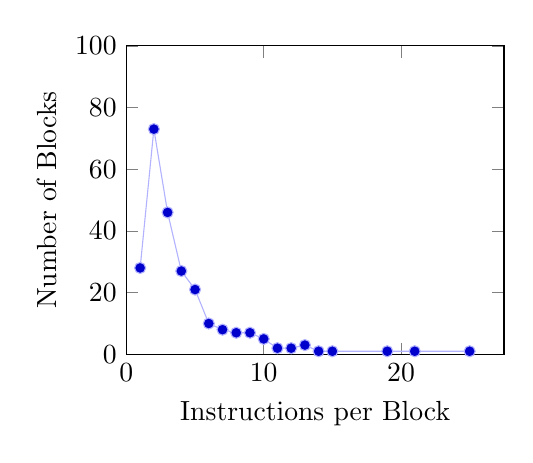
\begin{tikzpicture}
			\begin{axis}[
				xmin=0,
				ymin=0,
				ymax=100,
				height=5.5cm,
				xlabel={Instructions per Block},
				ylabel={Number of Blocks}
				%width=0.5\linewidth
			]
			\addplot+ [draw=oxtra-purple] coordinates {
				(1 ,28 )
				(2 ,73 )
				(3 ,46 )
				(4 ,27 )
				(5 ,21 )
				(6 ,10 )
				(7 ,8 )
				(8 ,7 )
				(9 ,7 )
				(10,5 )
				(11,2 )
				(12,2 )
				(13,3 )
				(14,1 )
				(15,1 )
				(19,1 )
				(21,1 )
				(25,1 )
			};
			\end{axis}
		\end{tikzpicture}
		\caption[Instructions per Block]{Primes, oxtra (b)}
		\label{fig:bench-block-prime-b}
	\end{subfigure}
	~
	\begin{subfigure}[t]{0.49\textwidth}
		\centering
		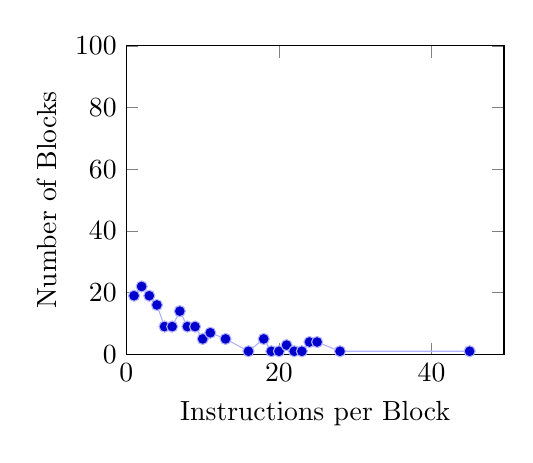
\begin{tikzpicture}
		\begin{axis}[
		xmin=0,
		ymin=0,
		ymax=100,
		height=5.5cm,
		xlabel={Instructions per Block},
		ylabel={Number of Blocks}
		%width=0.5\linewidth
		]
		\addplot+ [draw=oxtra-purple] coordinates {
			(1 ,19)
			(2 ,22)
			(3 ,19)
			(4 ,16)
			(5 , 9)
			(6 , 9)
			(7 ,14)
			(8 , 9)
			(9 , 9)
			(10, 5)
			(11, 7)
			(13, 5)
			(16, 1)
			(18, 5)
			(19, 1)
			(20, 1)
			(21, 3)
			(22, 1)
			(23, 1)
			(24, 4)
			(25, 4)
			(28, 1)
			(45, 1)
		};
		\end{axis}
		\end{tikzpicture}
		\caption[Instructions per Block]{Primes, oxtra (c)}
		\label{fig:bench-block-prime-c}
	\end{subfigure}
	~
	\begin{subfigure}[t]{0.49\textwidth}
		\centering
		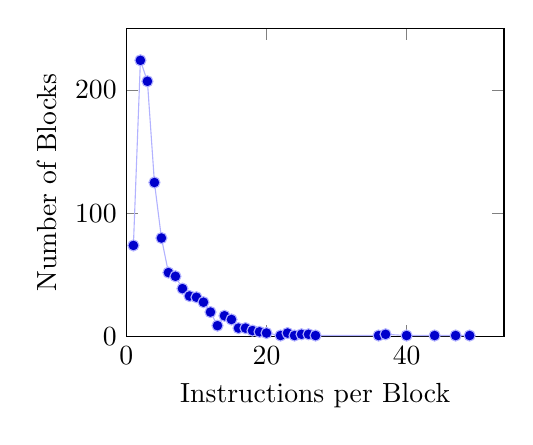
\begin{tikzpicture}
		\begin{axis}[
		xmin=0,
		ymin=0,
		ymax=250,
		height=5.5cm,
		xlabel={Instructions per Block},
		ylabel={Number of Blocks}
		%width=0.5\linewidth
		]
		\addplot+ [draw=oxtra-purple] coordinates {
			(1 ,74 )
			(2 ,224 )
			(3 ,207 )
			(4 ,125 )
			(5 ,80 )
			(6 ,52 )
			(7 ,49 )
			(8 ,39 )
			(9 ,33 )
			(10,32 )
			(11,28 )
			(12,20 )
			(13,9 )
			(14,17 )
			(15,14 )
			(16,7 )
			(17,7 )
			(18,5 )
			(19,4 )
			(20,3 )
			(22,1 )
			(23,3 )
			(24,1 )
			(25,2 )
			(26,2 )
			(27,1 )
			(36,1 )
			(37,2 )
			(40,1 )
			(44,1 )
			(47,1 )
			(49,1 )
		};
		\end{axis}
		\end{tikzpicture}
		\caption[Instructions per Block]{gzip, oxtra (b)}
		\label{fig:bench-block-gzip-b}
	\end{subfigure}	
	~
	\begin{subfigure}[t]{0.49\textwidth}
		\centering
		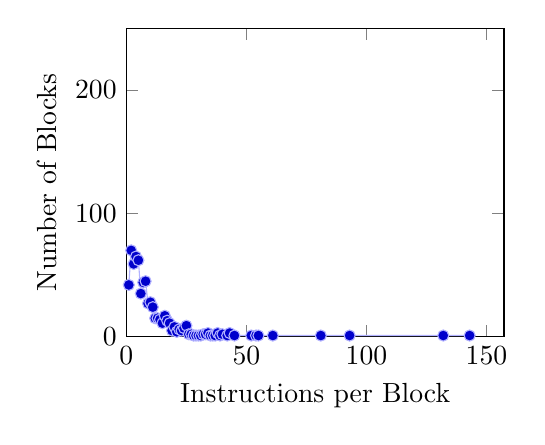
\begin{tikzpicture}
		\begin{axis}[
		xmin=0,
		ymin=0,
		ymax=250,
		height=5.5cm,
		xlabel={Instructions per Block},
		ylabel={Number of Blocks}
		%width=0.5\linewidth
		]
		\addplot+ [draw=oxtra-purple] coordinates {
			(1 ,42 )
			(2 ,70 )
			(3 ,59 )
			(4 ,65 )
			(5 ,62 )
			(6 ,35 )
			(7 ,44 )
			(8 ,45 )
			(9 ,27 )
			(10,28 )
			(11,24 )
			(12,15 )
			(13,15 )
			(14,14 )
			(15,11 )
			(16,17 )
			(17,13 )
			(18,11 )
			(19,5 )
			(20,8 )
			(21,4 )
			(22,6 )
			(23,5 )
			(24,7 )
			(25,9 )
			(26,2 )
			(27,2 )
			(28,1 )
			(29,1 )
			(30,1 )
			(31,1 )
			(32,2 )
			(33,2 )
			(34,3 )
			(35,1 )
			(36,1 )
			(37,1 )
			(38,3 )
			(39,1 )
			(40,2 )
			(42,1 )
			(43,3 )
			(45,1 )
			(52,1 )
			(54,1 )
			(55,1 )
			(61,1 )
			(81,1 )
			(93,1 )
			(132,1 )
			(143,1 )
		};
		\end{axis}
		\end{tikzpicture}
		\caption[Instructions per Block]{gzip, oxtra (c)}
		\label{fig:bench-block-gzip-c}
	\end{subfigure}
	\caption[Instructions per Block]{Occurrences of instructions per block (more instructions is better).}
\end{figure*}

% Limitations of testing
% Compare Prime test?
% Compare GZIP
% Compare memory, speed?
% Compare generation of instructions with qemu
% Generally compare with qemu

\subsection{Interpreting the Data}
The most striking feature of our dataset is oxtra's dwindling performance as inputs become less trivial. One possible explanation for this is the relatively low instruction density in the blocks we translate. Since oxtra does not retranslate any already translated code, it happens quite frequently, that a single instruction is executed, followed by a forced jump to the code which has already been translated.

Also of note is the considerable gain in performance observed after implementing a return stack. Doing so reduces the amount of necessary context switches, each of which would have necessitated loading and storing each register, a very time-consuming operation.

The performance increase resulting from recursive lookahead flag prediction is initially not as impressive as the one resulting from the return stack but becomes quite considerable as input sizes grow. This is likely due to the fact that only a few blocks are ever executed in a loop and decreasing the number of instructions generated for flag evaluation becomes more and more beneficial the more often that loop is executed.

\subsection{Possibility for Optimization}
% super blocks - less flag code
% translation process
% optimize blocks - problem: jumping to an instruction that was optimized
Considering that oxtra quickly becomes slower than QEMU as input become larger, there is still a lot to be done in the realm of optimization. Most importantly the translation process has a lot of potential.

One of the possible optimizations is to further optimize the blocks, for example by combining sequential \texttt{cmp} and \texttt{jcc} instructions into a single compare-and-branch instruction. However, this could lead to problems if the guest tries to jump to an instruction that was optimized away. In that case parts of that block would have to be translated again, which is not possible with our current code store architecture.

Another possible optimization would be to translate code multiple times. Even though this increases the time required to translate the code, it could yield an increase in execution speed as the number of static links on a path of blocks is reduced. This increase would be especially noticeable in frequently executed code such as conditional loops in the main execution cycle.

Another noteworthy optimization possibility is the strict rule of a block only having one entry. Currently the CodeStore allows blocks to have multiple entry and exit points, which prohibits optimizations within a block. If blocks were restricted to only having one single point of entry, the translated instructions could be optimized across each other. 

\subsection{Implementation Drawbacks and Trade-offs}
% free blocks - actual code cache
% allow guest to allocate new code
% allow guest to rewrite code
% code store page size - memory vs runtime
% call/ret optimization
% link oxtra statically - smaller binary size
% elf parser - allow dynamically linked executables (we can relocate it)
Many of the design decisions made during the development of oxtra come with their own characteristic downsides. First and foremost is our decision to store translated code indefinitely and optimize code generation based on that. Not only does this mean that we use more memory than if we had used a true code cache, it also prevents the guest from effectively utilizing self-modifying code since it would invalidate previously generated code. Depending on the extent of the modification large swaths of code would need to be retranslated even though oxtra is implemented on the assumption that code would only need to be translated once, as opposed to using a code cache, where self-modifying code could be dealt with by simply flushing the cache.

Another possibility for optimization is how large the pages oxtra uses internally to store generated code are. Smaller pages lead to more memory overhead but in turn improve execution time, since searching for addresses becomes easier, although adjusting this value often only has a small impact, since oxtra's code store uses binary search when looking up addresses.


\pagebreak
\section{Conclusion} % 1 Seite
% Oxtra ist geil und ist geil und fokusiert auf zwei architekturen
Oxtra's focus on two specific architectures enables it to outperform the leading competitor QEMU in many cases. 
In benchmarks performed against a QEMU emulation, oxtra is up to 20\% faster than QEMU when executing the command line tool gzip and generally outperforms QEMU when executing low to medium complexity programs. 
Notably, as the comparison is based on a QEMU emulation, the results might be different on real RISC-V hardware. 

For a rough indicator of performance on actual hardware, we also analyzed the number of generated instructions and actually executed instructions (including the instructions required for code translation). 
In our test suite, oxtra generates about 20\% fewer instructions than QEMU and executes about 10--40\% fewer instructions than QEMU.
With non-trivial input, the proportional advantage of oxtra over QEMU decreases but consistently remains above 10\%.
\\

\noindent Oxtra currently only supports a small subset of x86-64 instructions. 
Most notable is the lack of support for SSE instructions. While adding specific instructions of an already supported instruction set is straightforward, adding a completely new instruction set (extension) potentially requires modifying the core architecture.

As of now, oxtra is only able to translate statically linked Linux programs and is incapable of loading libraries at runtime.
This is prohibited by the internal structure of the code store. 
Additionally, multi-threaded programs and self-modifying code are not supported.

In oxtra, code can only be translated once.
This implies that instructions that logically belong to the same block but are translated later must be connected through static links. 
Allowing code to be translated again (replacing previous blocks) would solve this issue and is the next step for improving performance.
Flag evaluation can also be improved: Currently, the instruction that updates the flag stores information to memory and the instruction that uses the flag loads this information from memory before calculating the state. 
This can be avoided by evaluating the flag directly and is the more common case. 
\\

% was wären die nächsten logischen steps für oxtra (instruktionen hinzufügen etc.)
% also generell die zukunft
\noindent The current version of oxtra is limited in its capabilities but still proves to have a lot of potential and can be used as a starting point for a performant RISC-V binary translator.

\pagebreak
\printbibliography[heading=bibintoc,title={References}]

\pagebreak
\begin{appendices}
\section{Working with oxtra}
\label{Build Environment and Dependencies}
Oxtra is meant to be built as a 64 bit Linux ELF for RISC-V. This means, that it can only be used if RISC-V hardware is available\footnote{Oxtra has never been tested on real RISC-V hardware.} or an emulator is available. During development, we have used \emph{QEMU} with \emph{binfmt-support} installed alongside. All tools required for building and running oxtra are available as a Docker image: \texttt{plainerman/qemuriscv:oxtra}.

\subsection{Building and Testing}
In order to build oxtra, a C++ compiler for RISC-V (currently, only \emph{gcc} is supported) is required. Further, oxtra is a CMake project, hence requiring \emph{CMake} itself and a build tool to be installed alongside (e.g. \emph{make}).

With all the necessary requirements being installed and the git repository checked out, the CMake project can be initialized. Depending on preferences, the build type can be set to debug or release and a specific path for the RISC-V C/C++ compiler can be specified (required for building on a non-RISC-V computer). 

\begin{lstlisting}
$ cmake -D CMAKE_BUILD_TYPE=release \
 -D CMAKE_C_COMPILER=/opt/riscv/bin/riscv64-gnu-gcc \ 
 -D CMAKE_CXX_COMPILER=/opt/riscv/bin/riscv64-gnu-g++ .
\end{lstlisting}

Once the Makefile has been generated, oxtra can be built (including unit tests) by simply issuing the following command:

\begin{lstlisting}
$ make
\end{lstlisting}

Tests are not executed automatically during the build process and must be started manually. The unit tests are a self-contained binary (created by \emph{catch2}), but for the integration tests, \emph{shelltestrunner}\footnote{\url{https://github.com/simonmichael/shelltestrunner}} is required.

% Perl is only a hack, otherwise the /* would be interpreted as a comment
\begin{lstlisting}[language=Perl]
$ test/unit_tests
$ shelltest --all --timeout=30 --threads=4 test/integration/*.otest
\end{lstlisting}

\subsection{Using oxtra}
If QEMU is installed with binfmt-support (or you have a RISC-V 64 bit Linux), oxtra can be executed by simply invoking:
\begin{lstlisting}
$ ./oxtra path/to/x86-64-elf [-a "arguments"]
\end{lstlisting}

The above line executes the specified x86-64 elf binary and if arguments have been added, passes those to the guest application.

It is often useful to enable logging. Every logging type can be enabled/disabled separately. To enable all types, \(-1\) can be passed with:
\begin{lstlisting}
$ ./oxtra path/to/x86-64-elf [-a "arguments"] -l -1
\end{lstlisting}

If there is unexpected behavior, you can debug the execution by appending the debug flag and specifying the granularity (1 for debugging x86-64 instructions, 2 for RISC-V):
\begin{lstlisting}
$ ./oxtra path/to/x86-64-elf [-a "arguments"] --debug 1
\end{lstlisting}

Once the first basic block has been translated, you can enter "help" for more information. Additional resources on how to use the debugger can be found in \cref{Debugger}.
\\\\
\noindent For more information, you can consult the help page by entering:
\begin{lstlisting}
$ ./oxtra --help
\end{lstlisting}

\pagebreak
\section{Contribution}
Oxtra provides many highly optimized methods that enable the quick implementation of features (especially new instructions) without working on low-level RISC-V instructions directly. 
	
	\subsection{Helper Methods in Instruction}
	To ease the process of translating instructions, oxtra features a large set of helper functions. The most noteworthy are explained below.
	
	\subsubsection{translate\_operand}
	This function loads the operand at a given index into a register. It takes a lot of flags upon invoking, which ensure optimal code generation. As an example, there exists a flag that indicates to the function whether the resulting register should be modifiable or not or if the register should be loaded fully or only the operand size number of bits.
	
	\subsubsection{translate\_destination}
	This function is the counterpart to \texttt{translate\_operand}. It takes a register and stores it at the location described by the first operand of the instruction. It too comes with many flags indicating some features for optimizations.
	
	\subsubsection{read\_from\_memory and write\_to\_memory}
	These functions allow reading a certain value from memory into a register or writing it from a register into memory. They are used internally by \texttt{translate\_operand} and \texttt{translate\_destination}. In case of the destination being a memory address, both functions should be used, as they combine to make some optimizations, which otherwise would not be possible. 
	
	\subsubsection{translate\_memory}
	This function just computes a memory address and stores the result into a register passed to it. It is used internally by \texttt{read\_from\_memory and write\_to\_memory}.
	
	\subsubsection{call\_high\_level}
	This function allows for implementing very complicated logic in the generated code. It takes a callback to a static C or C++ function, which is invoked whenever the guest executes the corresponding instruction. The function works in the same way as the high-level evaluation for flags. Upon entry the function has access to the \texttt{ExecutionContext}, which contains all registers of the guest. The only modified register will be \texttt{RiscVRegister::t4}. The callback returns a 64 bit integer, which will be placed into register t4 before continuing execution of the generated code. 
	
	\subsubsection{load\_immediate}
	Loads a 64 bit immediate into a given register. The generated code aims at being the most efficient code to set the bits of the register the same way the immediate is set. 
	
	\subsubsection{load\_address}
	Loads a 64 bit address into a given register. The generated code will always consist of 8 instructions. This function is required by \texttt{reroute\_static} as it will overwrite the address it has been called from. If the previous address is shorter to encode than the new address, \texttt{reroute\_static} would run out of space to generate the new code.
	
	\subsubsection{append\_eob}
	Used by instructions that end the current block to append the code to call \texttt{reroute\_static} or \texttt{reroute\_dynamic}. Uses \texttt{load\_address} and the \texttt{jump table} internally.
	
	\subsection{Exiting the Guest}
	In the rare event that an error occurs, either in the code generation or in a high-level function written for the execution or for the flags, the generating code can exit the guest at any time. The dispatcher offers the functions \texttt{guest\_exit} and \texttt{fault\_exit}. Invoking these functions will restore the host context and exit the program. While both functions take a 64 bit value as return value, \texttt{fault\_exit} also takes a string pointer. This string will be printed as reason for the fault if the function is invoked.

\pagebreak
\section{Supported Instructions}
\label{Supported Instructions}
\[\begin{array}{llllll}
\texttt{adc} &
\texttt{add} &
\texttt{and} &
\texttt{bt} &
\texttt{btc} &
\texttt{btr} \\
\texttt{bts} &
\texttt{call} &
\texttt{cbw} &
\texttt{cdqe} &
\texttt{clc} &
\texttt{cmovcc} \\
\texttt{cmp} &
\texttt{cmps} &
\texttt{cwd} &
\texttt{cwde} &
\texttt{cdq} &
\texttt{cqo} \\
\texttt{dec} &
\texttt{div} &
\texttt{idiv} &
\texttt{imul} &
\texttt{inc} &
\texttt{jcc} \\
\texttt{jmp} &
\texttt{lea} &
\texttt{leave} &
\texttt{lods} &
\texttt{mov} &
\texttt{movs} \\
\texttt{movsx} &
\texttt{movzx} &
\texttt{mul} &
\texttt{neg} &
\texttt{nop} &
\texttt{not} \\
\texttt{or} &
\texttt{pop} &
\texttt{push} &
\texttt{ret} &
\texttt{rol} &
\texttt{ror} \\
\texttt{sar} &
\texttt{scas} &
\texttt{setcc} &
\texttt{shl} &
\texttt{shr} &
\texttt{stc} \\
\texttt{stos} &
\texttt{sub} &
\texttt{syscall} &
\texttt{test} &
\texttt{xor} &
\end{array}\]
\end{appendices}

\end{document}
